%!TEX root = ../dissertation.tex
\begin{savequote}[75mm]
You gotta have a swine to show you where the truffles are.
\qauthor{Edward Albee}
\end{savequote}

\chapter{Event Selection}
\label{sec:selection}

\begin{figure}[htbp!]
  \centering
  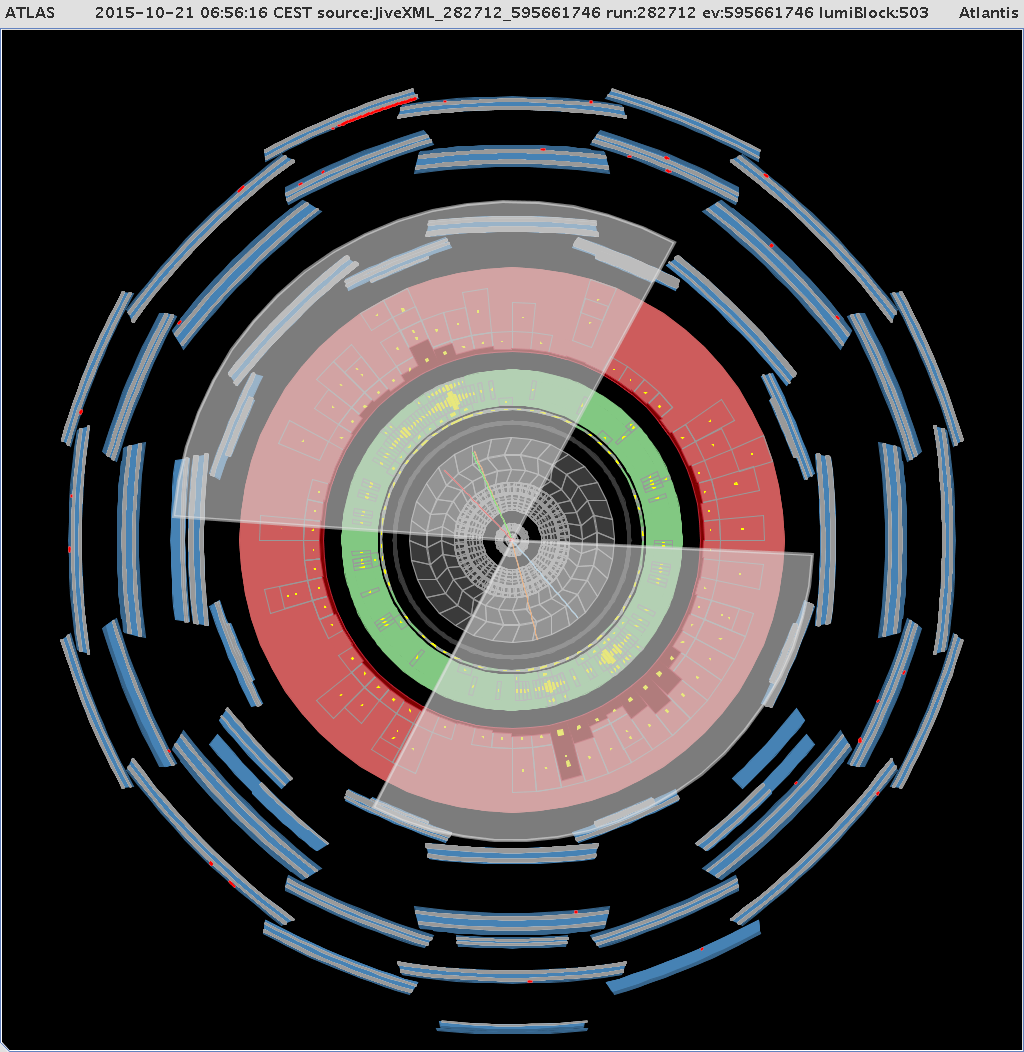
\includegraphics[width=0.7\textwidth]{figures/theory/JiveXML_282712_595661746-YX-2018-04-16-20-50-34}
  \caption{2015 ATLAS boosted di-Higgs event candidate's event display. The data is taken in run 282712, lumiblock 503 and has event number 595661746. ID is in gray, ECAL is in green, HCAL is in red and MS is in blue. Only tracks with \pt $>25$ \GeV are shown. Jets are gray cones, and ID tracks are colored lines in the ID. There are $2b$ tagged tracks within in each of the large-\R jets. The one large-\R jet has $119$ \GeV mass and $543$ \GeV \pt, and the other one has $127$ \GeV mass and $413$ \GeV \pt. The $\Delta R$ between the two large-\R jet is $3.54$ and the invariant mass of the two large-\R jets is $1336$ \GeV. }
  \label{fig:event_display}
\end{figure}

\paragraph{}
An example of \Xtohhb~ boosted event is shown in Figure~\ref{fig:event_display}. This chapter explains how this event is selected as a \Xtohhb~ candidate.

\section{Data Cleaning}
\label{evt-sel:cleaning}
\paragraph{}
The following data cleaning requirements are made:
\begin{itemize}
\item Events with problems in SCT/TileCal/LAr are removed.
%\item Events that are affected by the recovery procedure for single event upsets in the SCT are removed.
\item Events that fail the jet cleaning procedure are removed. This is designed to exclude jets caused by detector noise, non-collision backgrounds and cosmic rays. 
\item Incomplete events are removed.
\end{itemize}
% \paragraph{}
% Jets with $p_T<60$~\GeV\, $|\eta|<2.4$, and with a large fraction of their energy arising from pile-up interactions are suppressed using tracking information. 
% Events that pass a ``medium'' jet vertex tagger working point, corresponding to a 92\% efficiency for jets at the EM scale with $20<p_T<60$~\GeV, are retained in the analysis. 
% Quality criteria are applied to the jets, and events with jets consistent with noise in the calorimeter or non-collision backgrounds are vetoed~\cite{jetcleanATLAS}.
\paragraph{}
The analysis also runs over the debug stream, which contains events recorded that couln't be reconstructed on-line due to CPU time constrains. No event passing the full signal selection is found.


%%%%%%%%%%%%%%%%%%%%%%%%%%%%%%%%%%%%%%%%%%%%%%%%%%%%%%%%%%%%%%%%%%%%%%%%%%%%%%%%%%%%%%%%%%
\section{Trigger}
\label{evt-sel:trig}
\paragraph{}
%See \href{https://arxiv.org/pdf/1611.09661.pdf}{6.4.3} 
Events in data and MC are required to pass the lowest unprescaled large-\R jet trigger: \\
\verb|HLT_j360_a10_lcw| in 2015 and \verb|HLT_j420_a10_lcw| in 2016. 
The triggered jets are topo-cluster jets with local calibration weights and pile-up subtraction.
They are seeded by the lowest unprescaled L1 jet trigger, \texttt{L1\_J100}. 
LCW cluster trigger is chosen, because the other option, reclusted large-\R jet trigger, has slower turn-on in multi-jet events. 
Other options such as the lowest unprescaled HT trigger, \verb|HLT_ht1000|, has a much slower turn-on compared to large-\R jet triggers.
Another trigger option is \verb|HLT_4j100|, but because of the boosted jets merging, the trigger efficiency decreases rapidly as the signal mass increases. 
The results are shown in Figure~\ref{fig:boosted-trigger-HLT}.

\begin{figure}[htbp!]
\begin{center}
  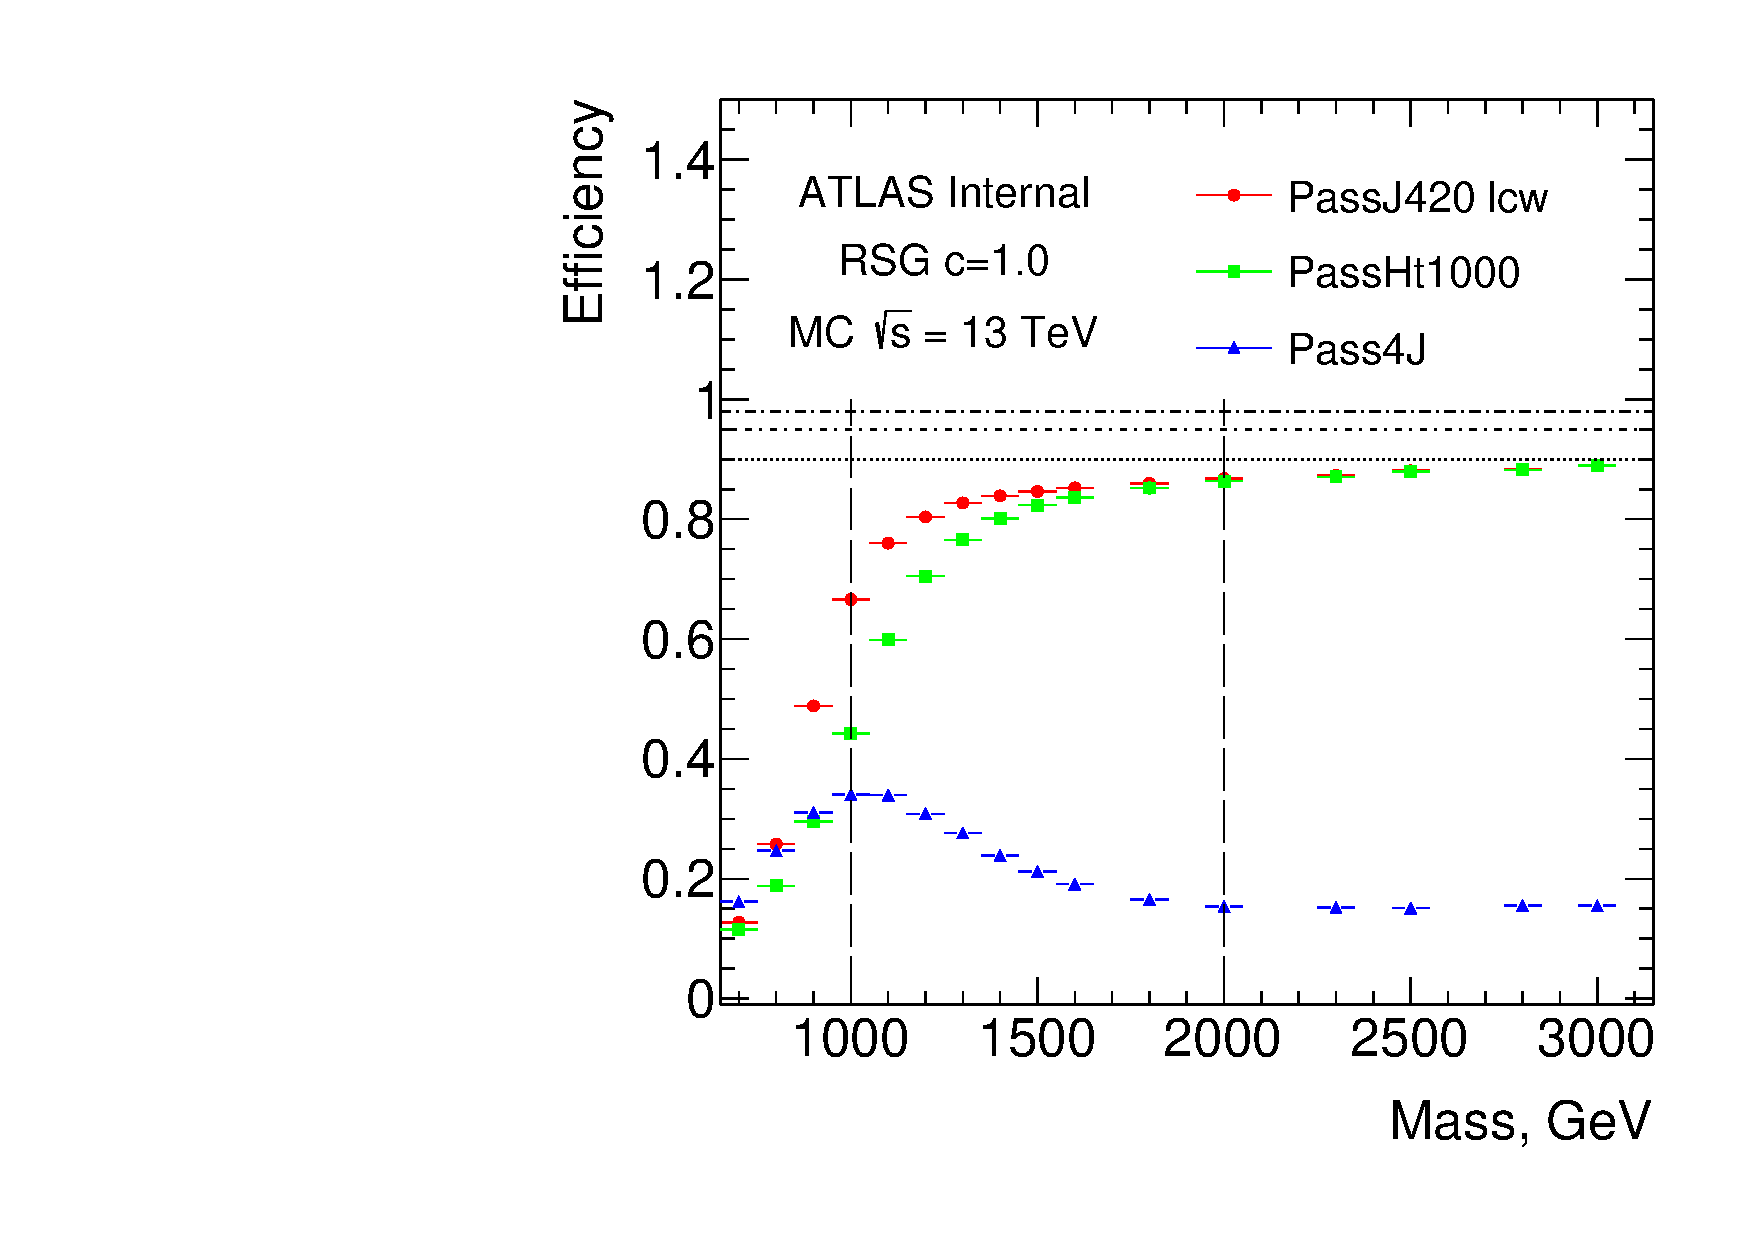
\includegraphics[width=0.45\textwidth,angle=-90]{figures/boosted/Trigger/app_trig_b77_Efficiency_PreSel.pdf}
  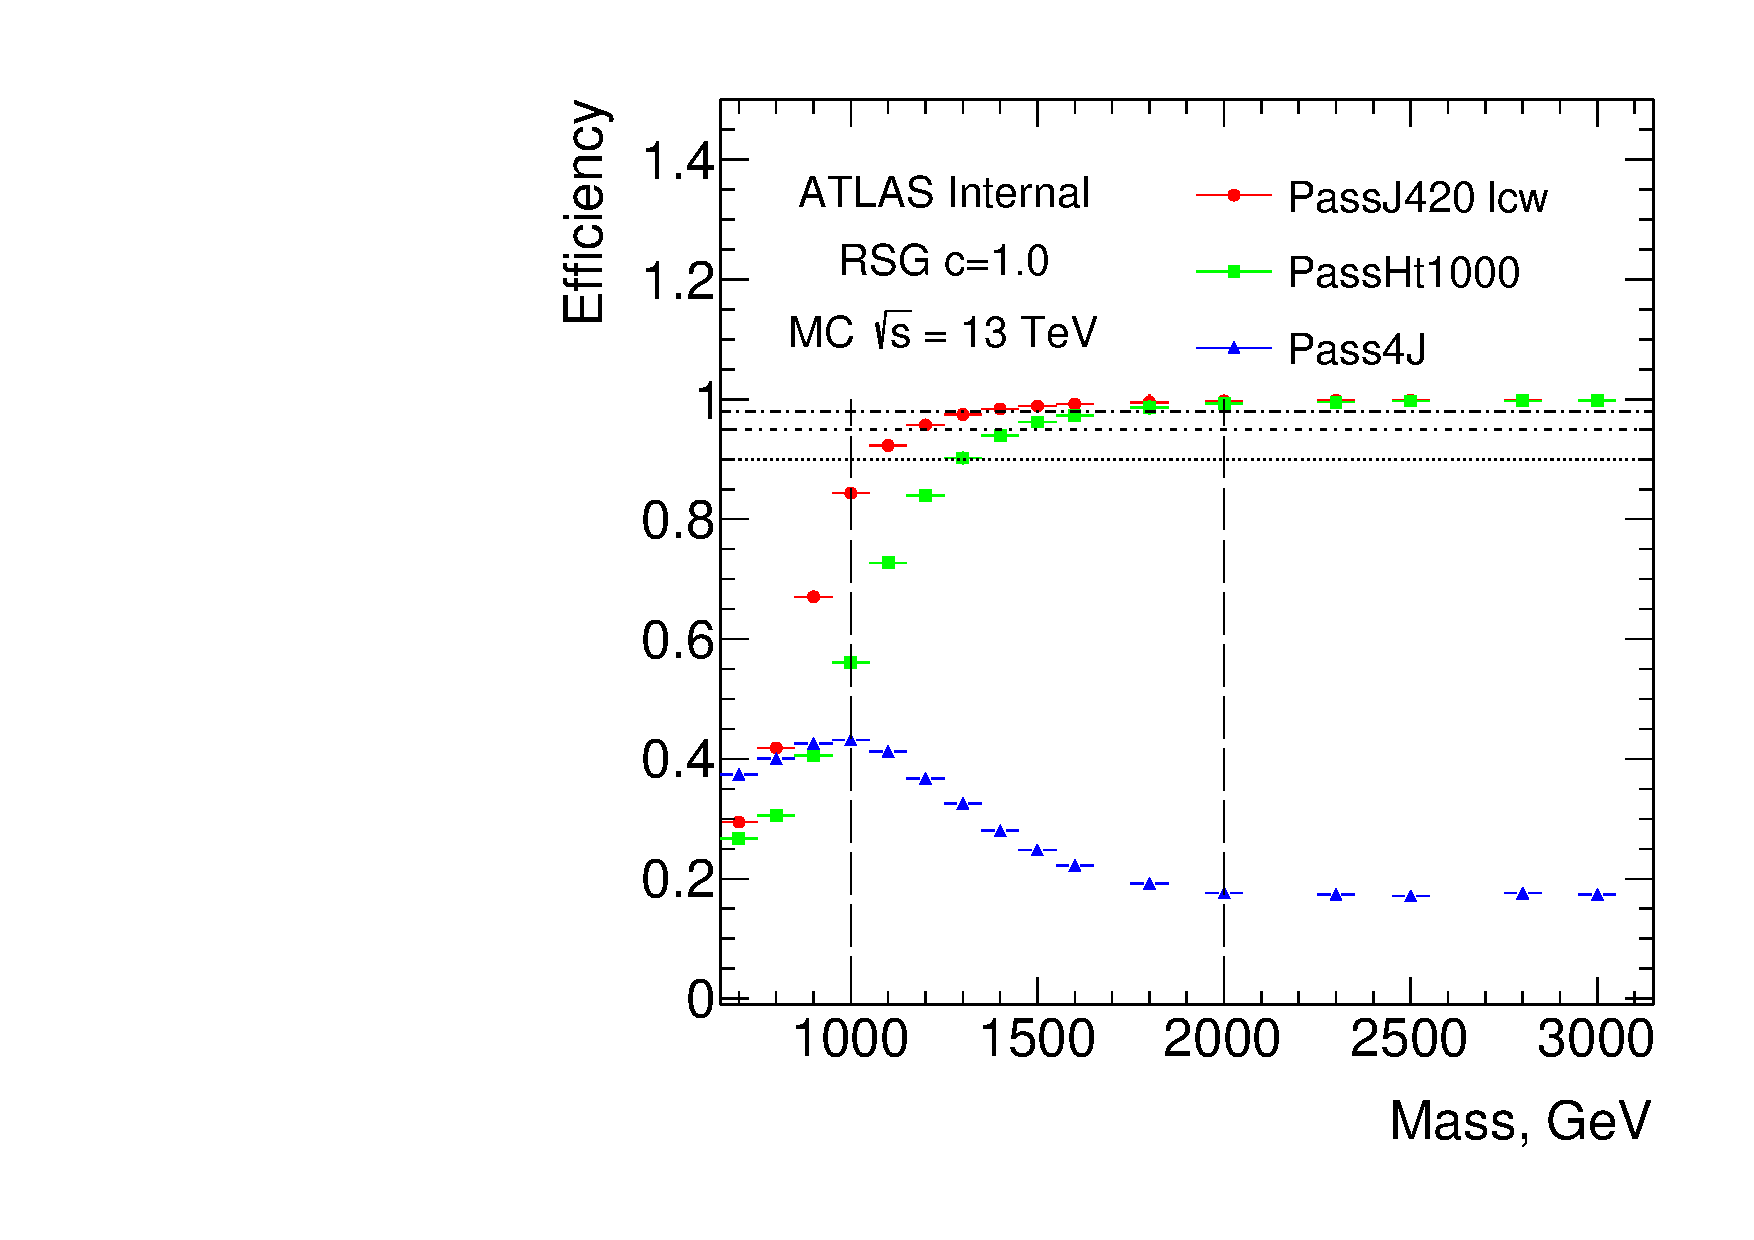
\includegraphics[width=0.45\textwidth,angle=-90]{figures/boosted/Trigger/app_trig_b77_Efficiency_All.pdf}
  %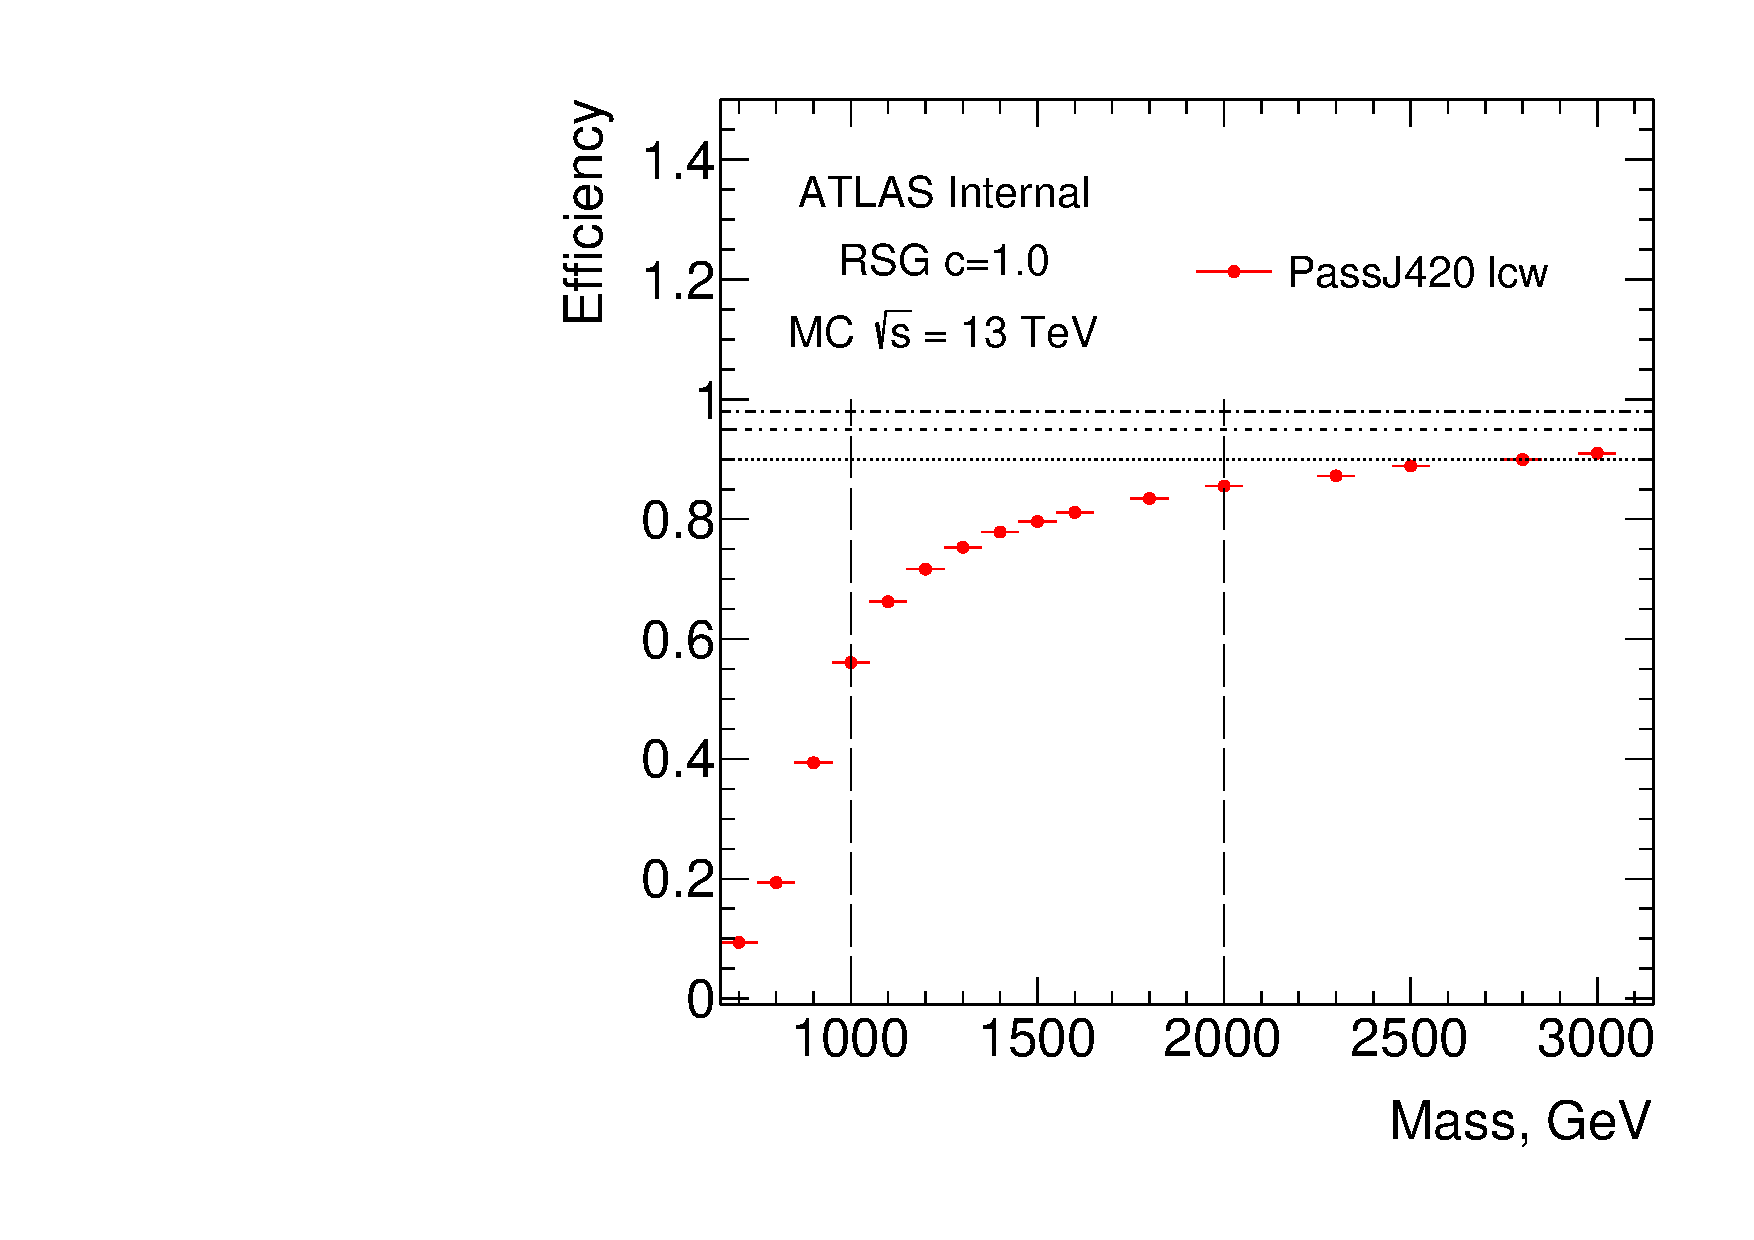
\includegraphics[width=0.45\textwidth,angle=-90]{figures/boosted/Trigger/trig_Moriond_Efficiency_PreSel.pdf}
  %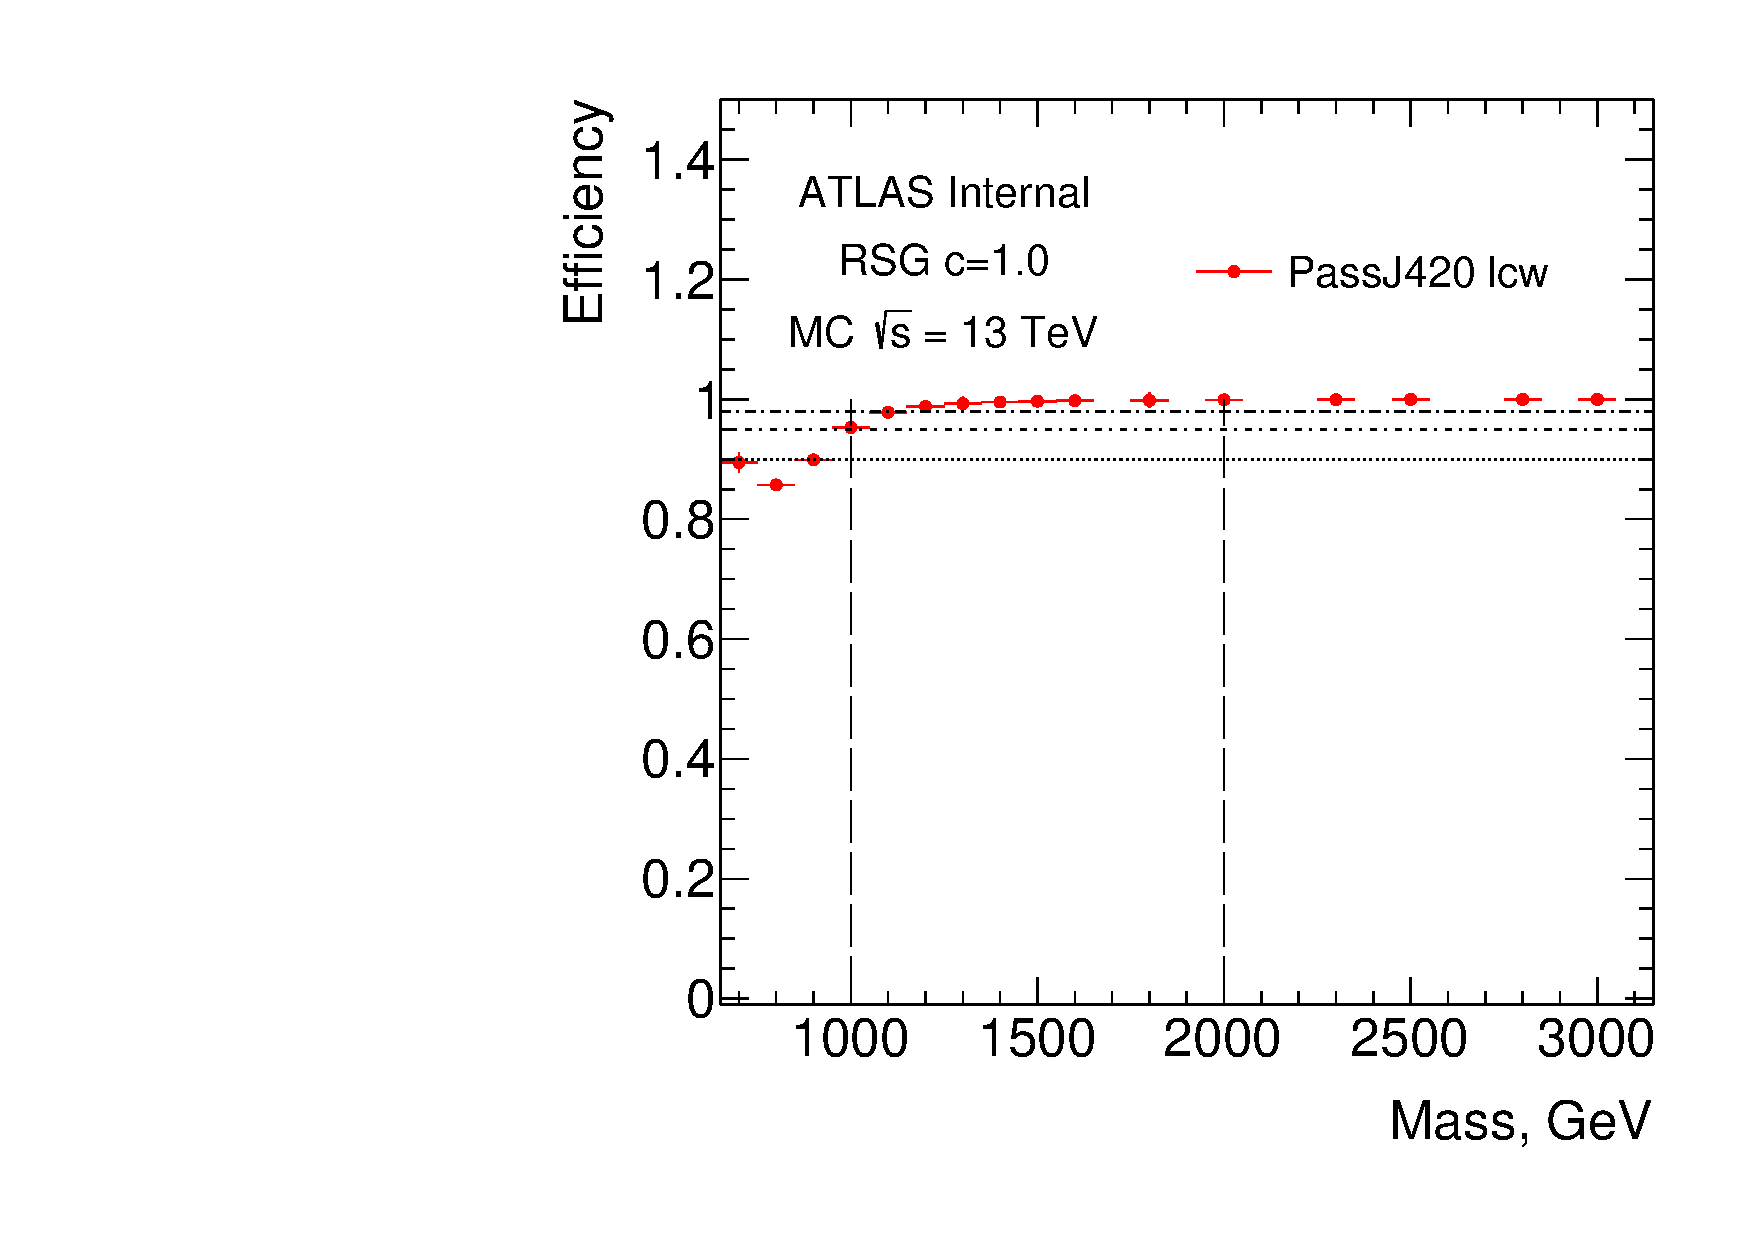
\includegraphics[width=0.45\textwidth,angle=-90]{figures/boosted/Trigger/trig_Moriond_Efficiency_All.pdf}
  \caption{Different trigger efficiencies as a function of the signal resonance mass with respect to all events with no selection (left) and with respect to events passing the two large-\R jets \pt $> 400$ \GeV~ and leading/subleading jet \pt $> 250$ \GeV (right). For $1.4$ \TeV~ signal, the trigger efficiency is about $98\%$.}
  \label{fig:boosted-trigger-HLT}
\end{center}
\end{figure}

\paragraph{}
The selected large-\R triggers are found to have $>98\%$ efficiency for signals with mass above 1400 \GeV.
% with the requirement that the event has two large-\R jets that satisfy the \pt requirements: leading jet \pt $> 400$ \GeV, and subleading jet leading jet \pt $> 250$ \GeV. 
The trigger turn-on curve in 2015 and 2016 data, as a function of leading jet \pt, is shown in Figure~\ref{fig:boosted-trigger-HLT-turnon}.
\begin{figure}[htbp!]
\begin{center}
  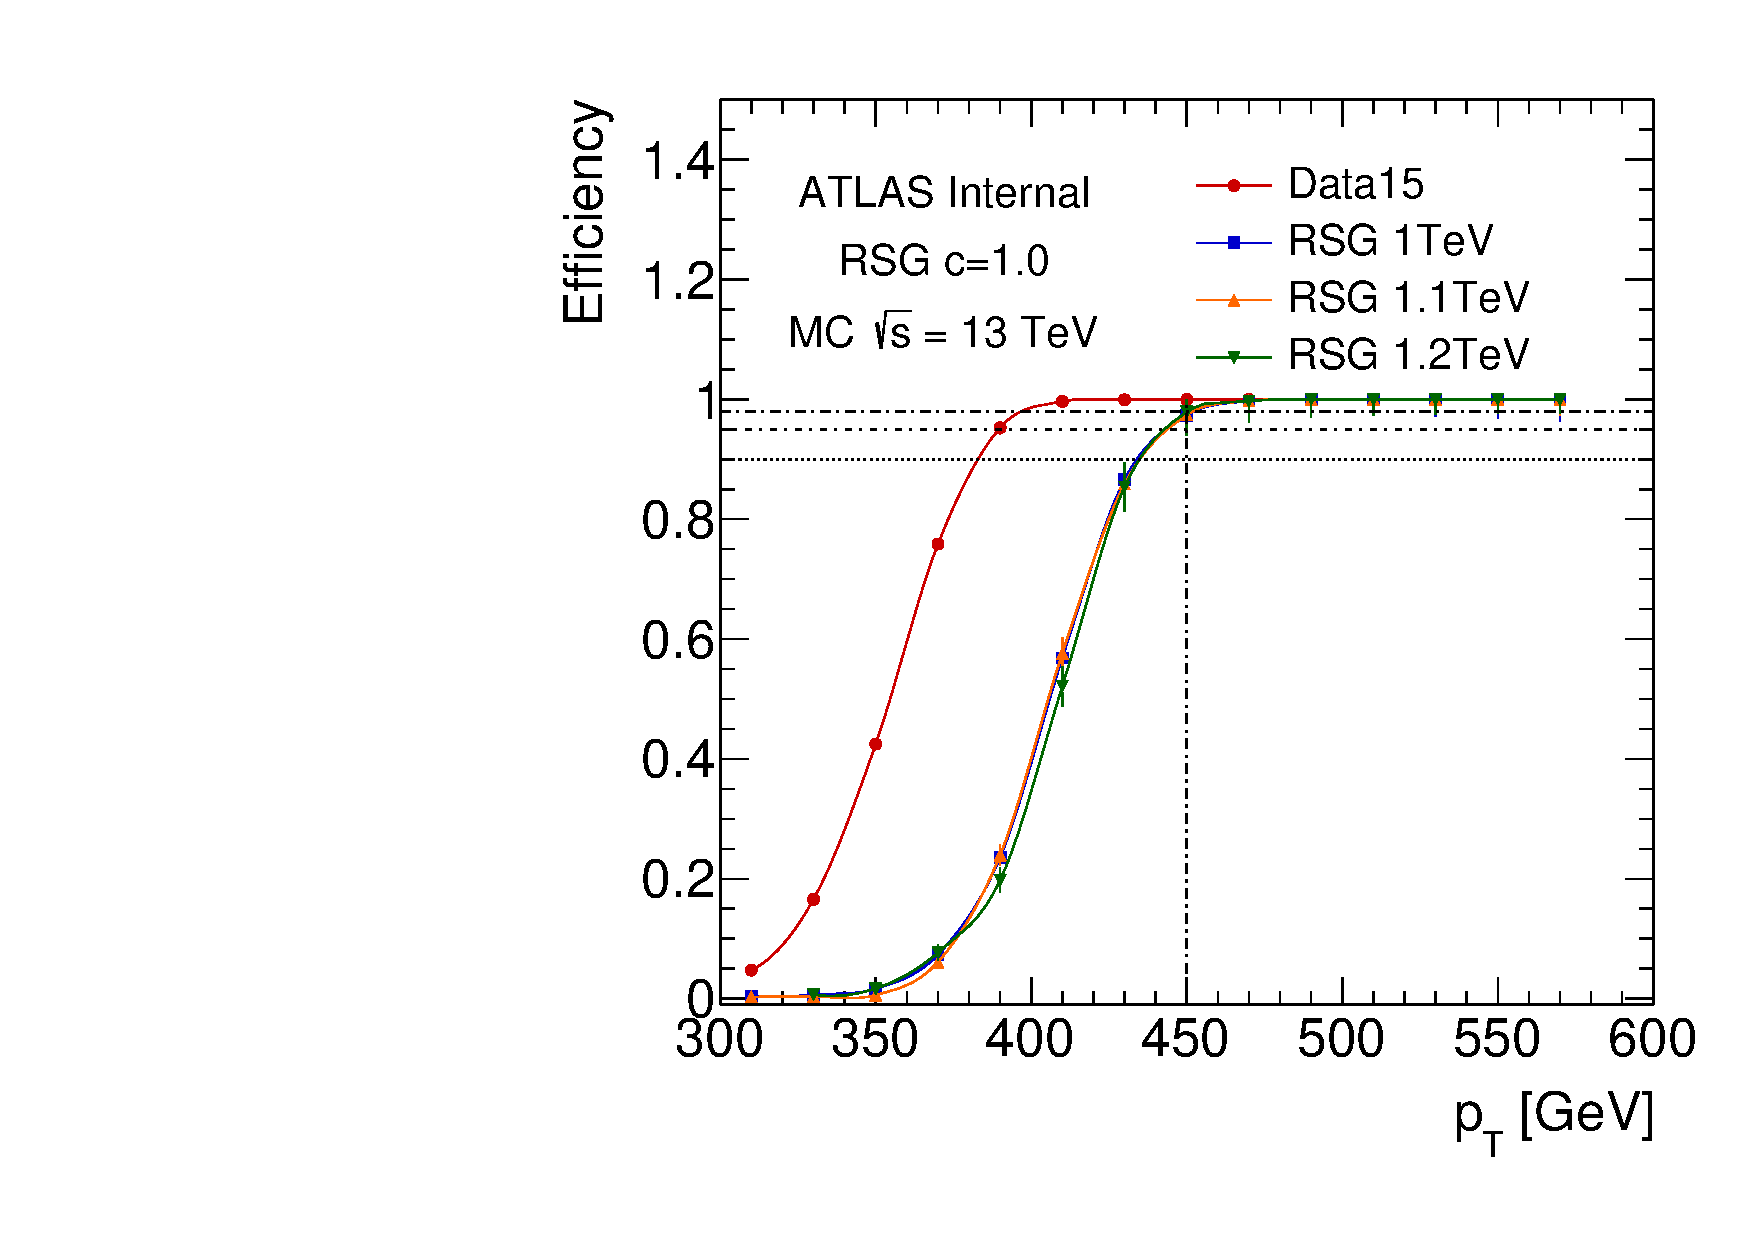
\includegraphics[width=0.45\textwidth,angle=-90]{figures/boosted/Trigger/trig_15_b77_pT_Efficiency.pdf}
  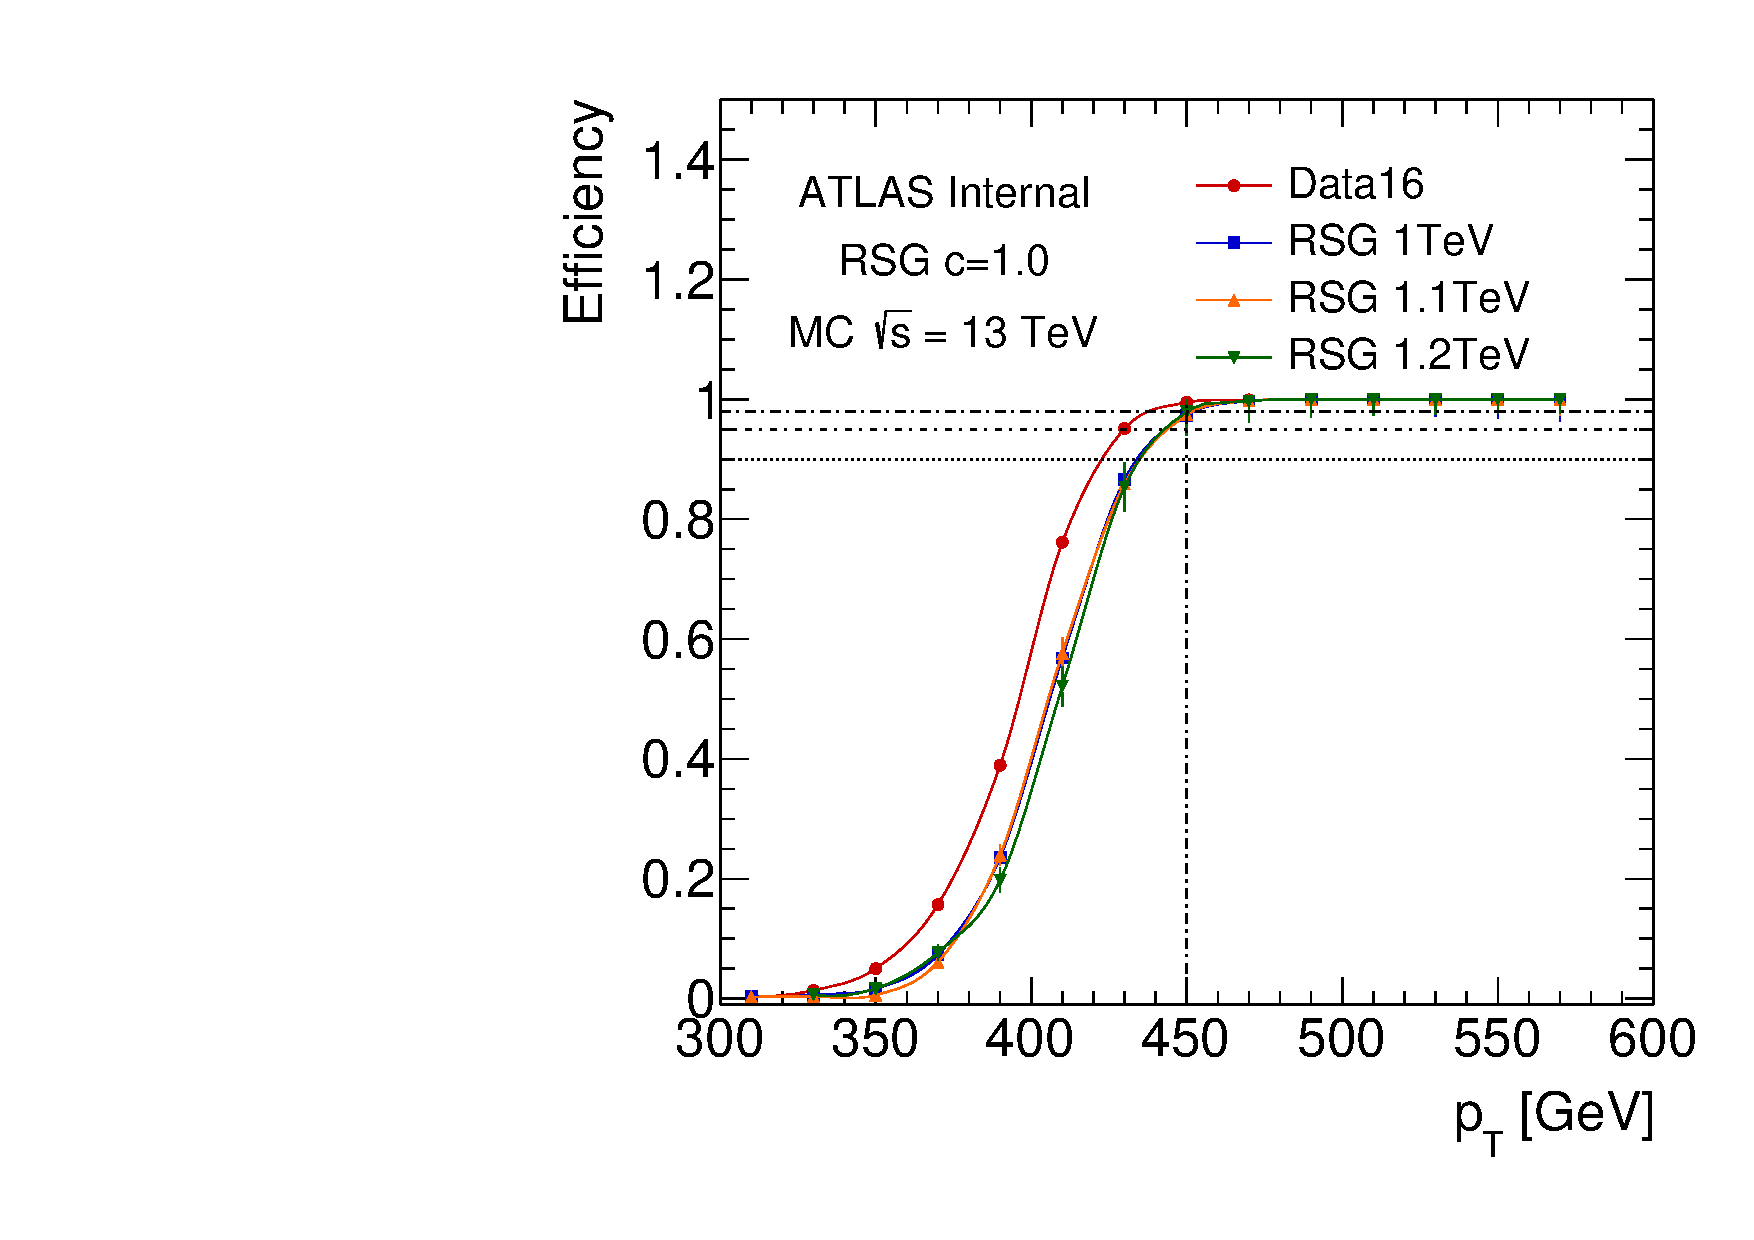
\includegraphics[width=0.45\textwidth,angle=-90]{figures/boosted/Trigger/trig_16_b77_pT_Efficiency.pdf}
  \caption{Large-$R$ jet trigger efficiencies, defined as the fraction of events fired trigger with a given highest large-\R jet \pt, measured in 2015 Data (\texttt{HLT\_j360\_a10\_lcw}, left) and 2016 Data (\texttt{HLT\_j420\_a10\_lcw}, right) and MC.}
  \label{fig:boosted-trigger-HLT-turnon}
\end{center}
\end{figure}


%%%%%%%%%%%%%%%%%%%%%%%%%%%%%%%%%%%%%%%%%%%%%%%%%%%%%%%%%%%%%%%%%%%%%%%%%%%%%%%%%%%%%%%%%%
\section{Object Selection}
\paragraph{}
The specific physics objects used in the boosted analysis are described in previous sections and reiterated in Table~\ref{tab:boosted-objects}.

\begin{table}[bhp]
\caption{Physics objects and their technical names in the boosted analysis.} %%%
\begin{center}
\begin{tabular}{c|c}
  object & technical name \\
  \hline
  large-$R$ calorimeter jets & AntiKt10LCTopoTrimmedPtFrac5SmallR20Jets \\
  small-$R$ track jets       & AntiKt2PV0TrackJets \\
  b-tagging                  & on track jets, MV2c10, $70\%$ b-tagging wp \\
\end{tabular}
\label{tab:boosted-objects}
\end{center}
\end{table}

\paragraph{}
Each event must have at least two high momentum large-\R jets, each with at least one ghost associated track jets for $b$-tagging.
They are sorted by \pt, and the highest \pt~ one is named as the leading large-\R jet, or the leading Higgs Candidate.
The second highest \pt~ large-\R jet is the subleading large-\R jet, or the subleading Higgs Candidate.
The large-\R jets are required to have \pt $> 250$ \GeV~, $|\eta| < 2$ to guarantee a good overlap with the tracking acceptance, and mass $> 50$ \GeV~ to avoid over-sized derivations.
The leading large-\R jet is also required to have \pt $> 450$ \GeV~ to be above the trigger turn on threshold.
Only the leading and subleading large-\R jets are considered in the rest of this thesis.
This selection is $\sim 95\%$ efficient for $1.2$ \TeV signals, as shown in Figure~\ref{fig:truth-Higgs-largeRjet}. 
$R = 1.0$ ensures that the two $b$ quarks and their decay products are very likely to be contained within the large-\R jet, as shown in Figure~\ref{fig:truth-HbdR}. 

\begin{figure}[htbp!]
	\begin{center}
	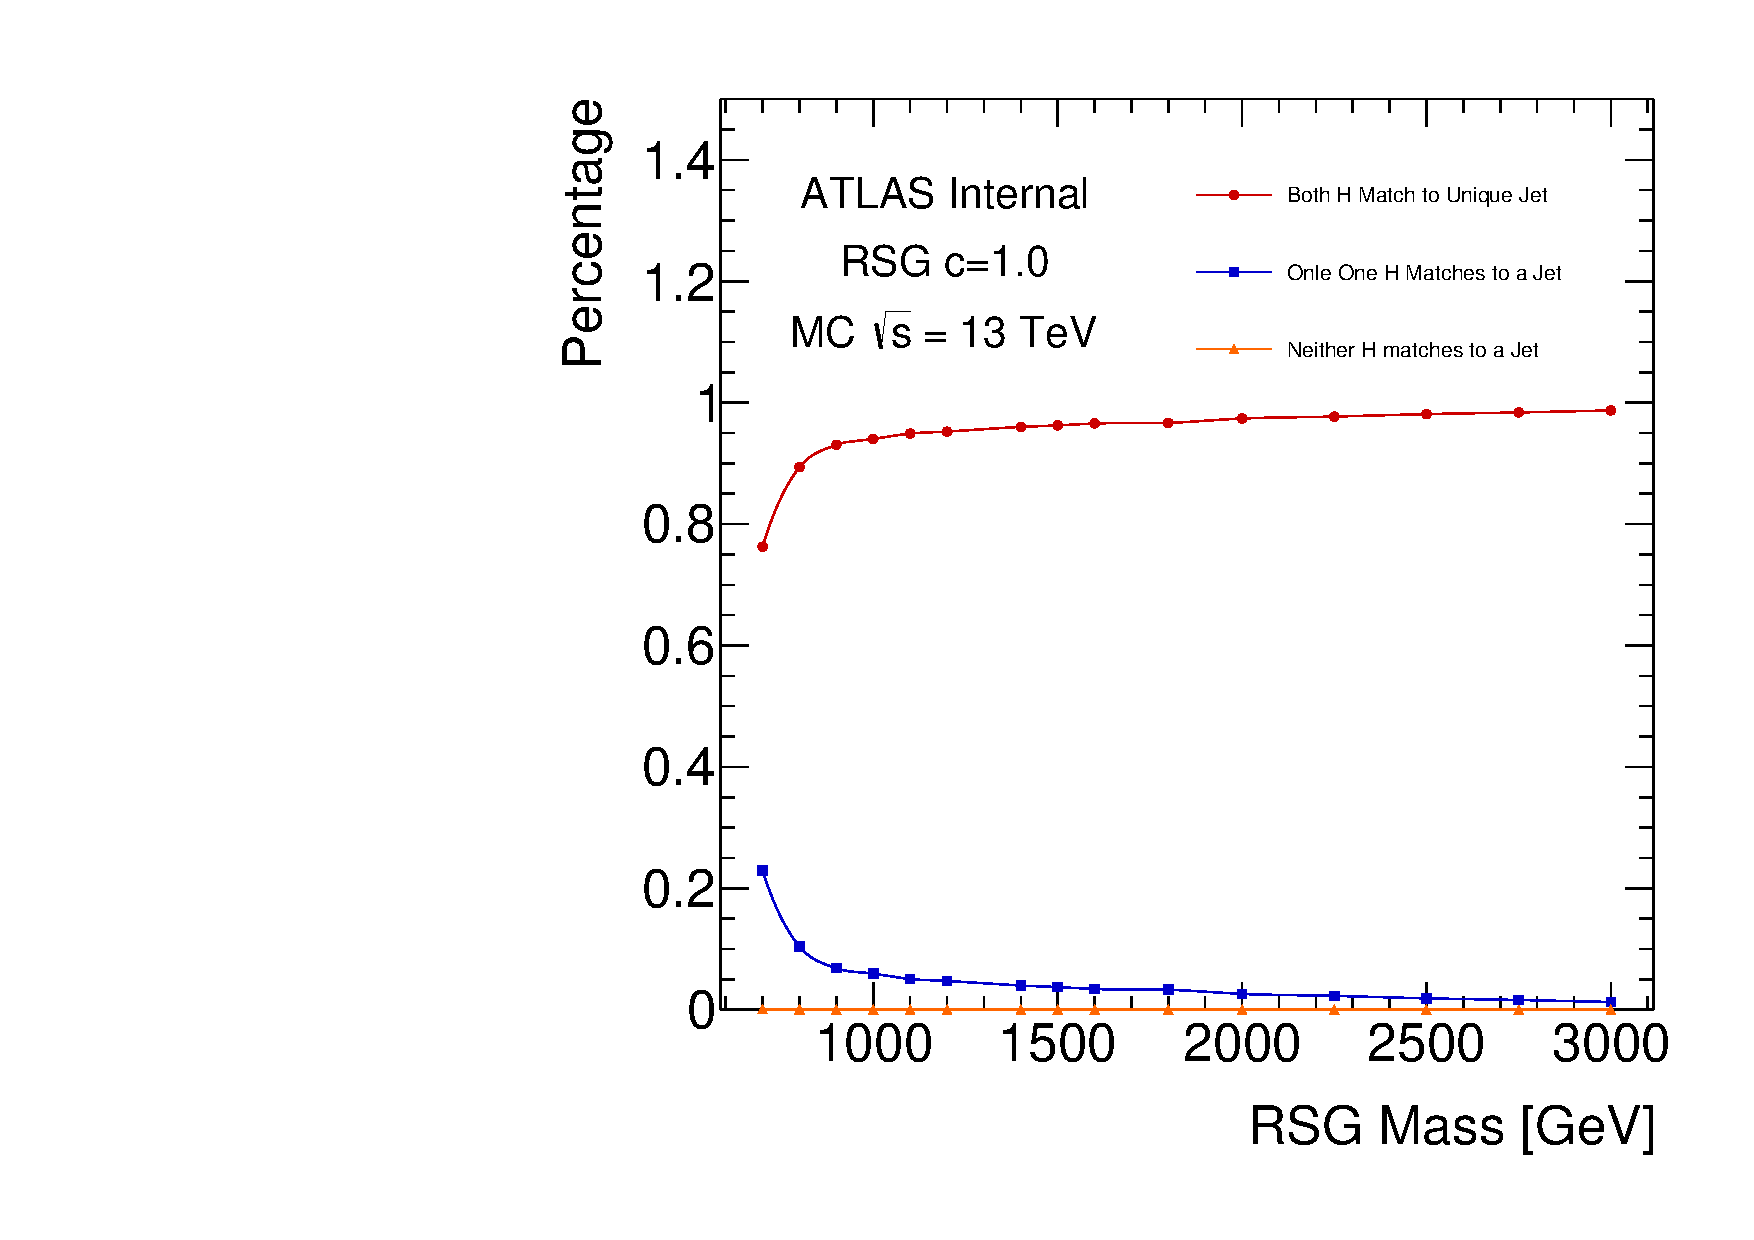
\includegraphics[scale=.45,angle=-90]{figures/boosted/Truth/truth_higgs-matching.pdf}
	\caption{Percentages of truth Higgs to large-\R jet $\Delta R<1.0$ matching as a function of \Grav~ mass. Both Higgs almost never match to the same large-\R jet.}
	\label{fig:truth-Higgs-largeRjet}
\end{center}
\end{figure}

\begin{figure}[htbp!]
\begin{center}
  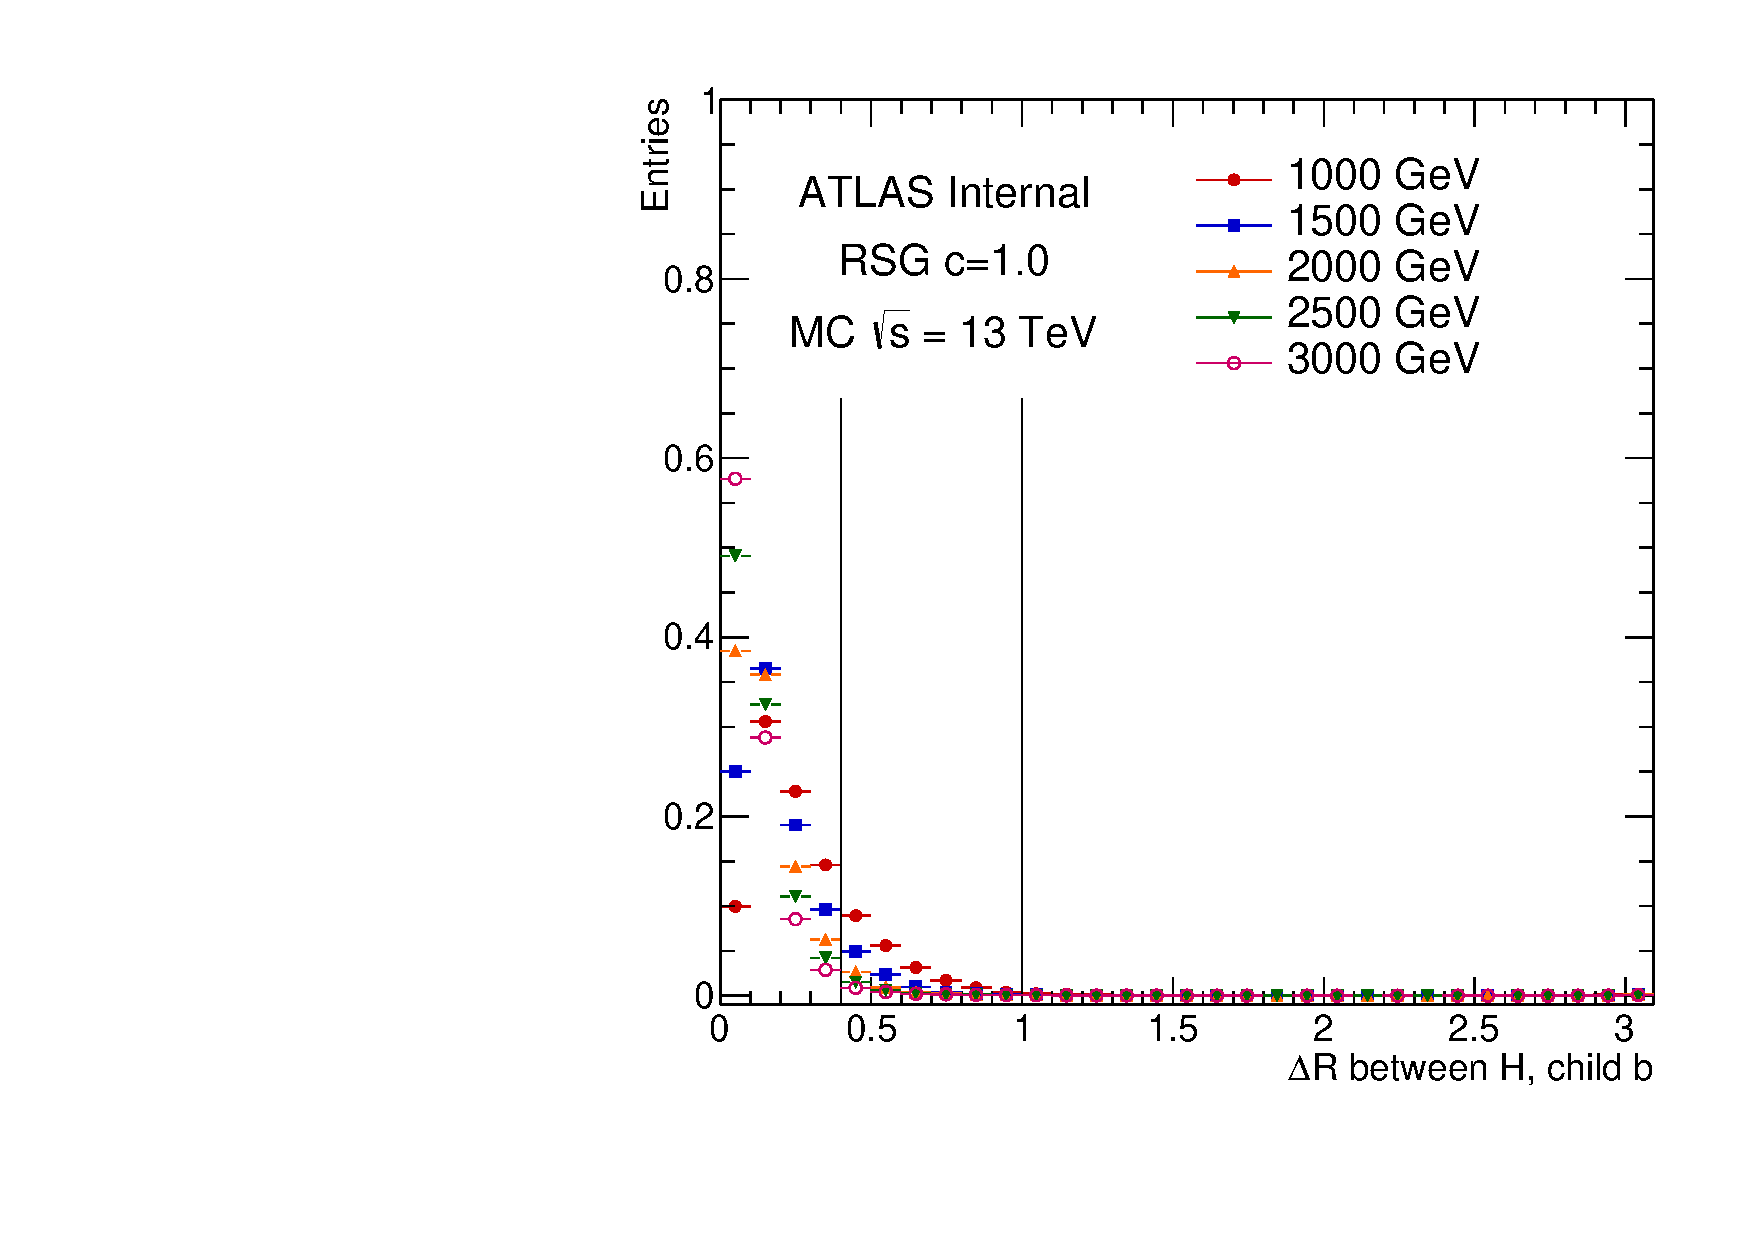
\includegraphics[width=0.45\textwidth,angle=-90]{figures/boosted/Truth/truth_hbdR.pdf}
  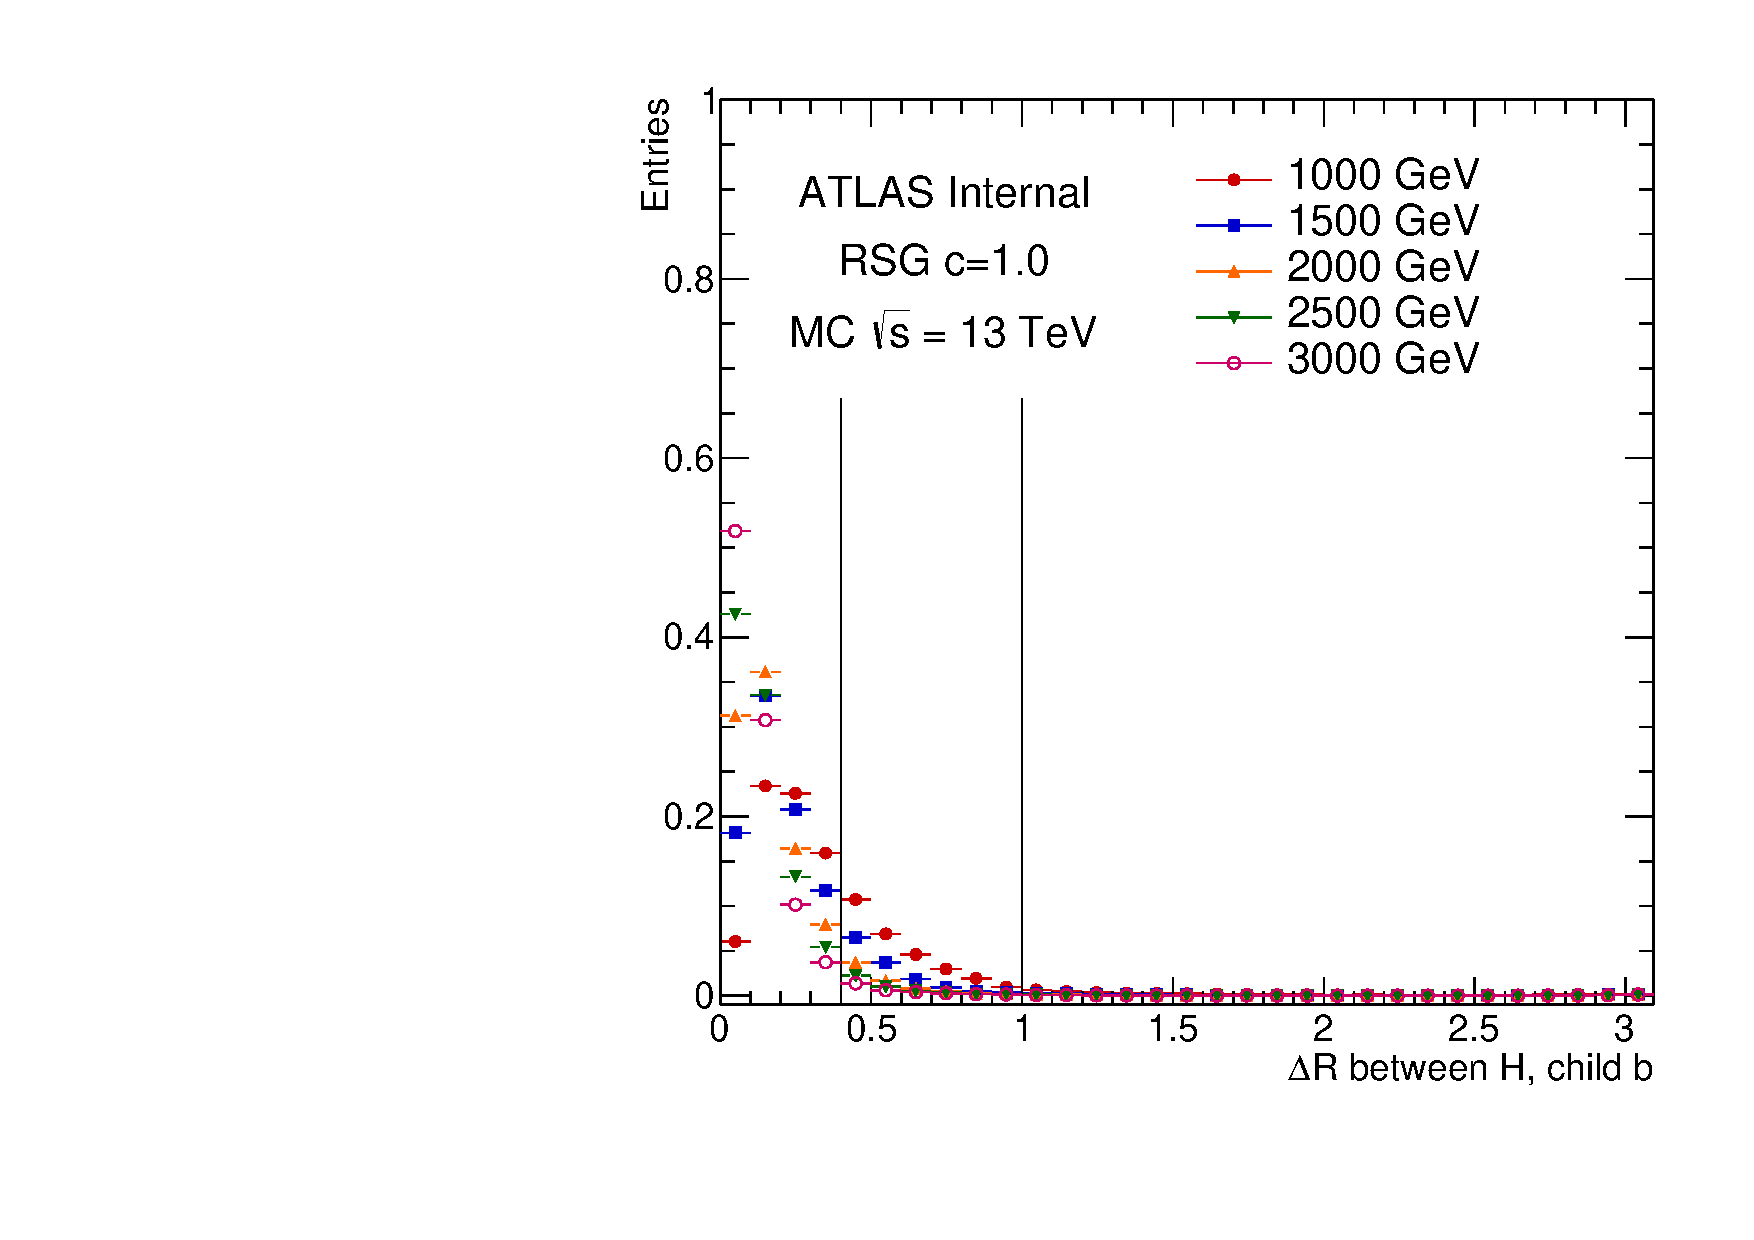
\includegraphics[width=0.45\textwidth,angle=-90]{figures/boosted/Truth/truth_hbdR2.pdf}
\caption{Normalized $\Delta R$ between the truth Higgs (leading on left, subleading on right) and the truth children $b$-quarks for \Grav~ MCs. Lines are drawn at $\Delta R = 0.4$ ($R$ of small-\R jets) and $\Delta R = 1.0$ ($R$ of large-\R jets). }
\label{fig:truth-HbdR}
\end{center}
\end{figure}

\paragraph{}
The track jets are required to have \pt $> 10$ \GeV, $|\eta| < 2.5$ and at least two tracks associated with it. 
A track jet is considered $b$-tagged if it has MV2c10 > $0.6455$, see Section~\ref{sec:btag_70wp} for details. 
Each large-\R jet is required to have at least one, not two, track jet Ghost associated with it.
This accounts for the $R=0.2$ track jets merging at really high boost, from signals above $2.5$ \TeV.
If there are more than one track jet contained in the large-\R jet, they are also sorted by \pt.
The highest \pt~ track jet is named as the leading track jet, and the second highest \pt~ one is named as the subleading track jet.
Only the two highest \pt~ track jet is considered in this thesis.
The one or two track jets $\Delta R$ match to the truth $b$ quarks $80\%$, as shown in Figure~\ref{fig:truth-bmatch}. 
In the Figure, red means the truth Higgs doesn't match the large-\R jet. Blue means both truth $b$ matches the two track jets. Orange means two truth $b$ matches one same track jet. Green indicates one $b$ quark has $\Delta R<0.2$ for both leading and subleading track jet, and the other $b$ is matched to one of the two track jets. Pink means one $b$ quark matches to one of the two track jets, the other $b$ doesn't match to the two leading track jets.

\begin{figure}[htbp!]
\begin{center}
  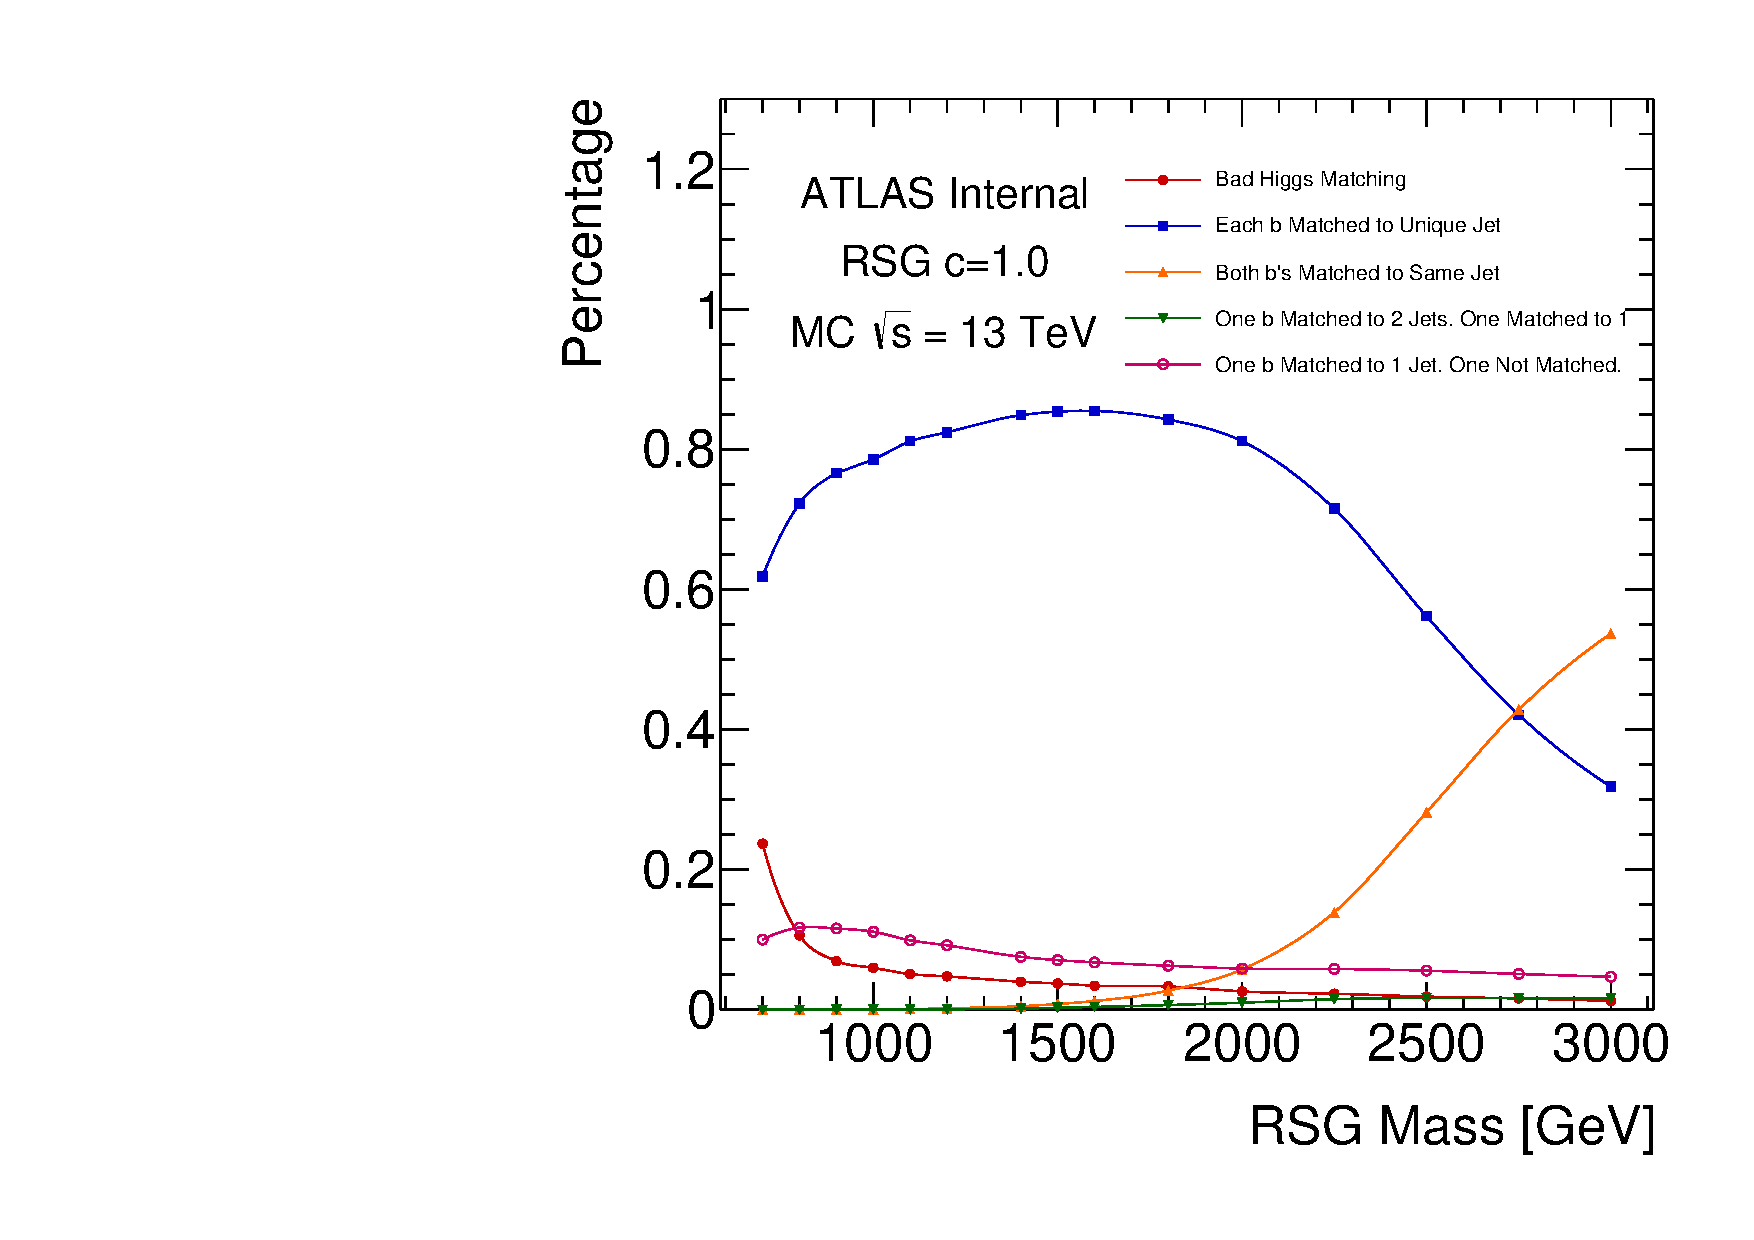
\includegraphics[width=0.45\textwidth,angle=-90]{figures/boosted/Truth/truth_b-matching.pdf}
  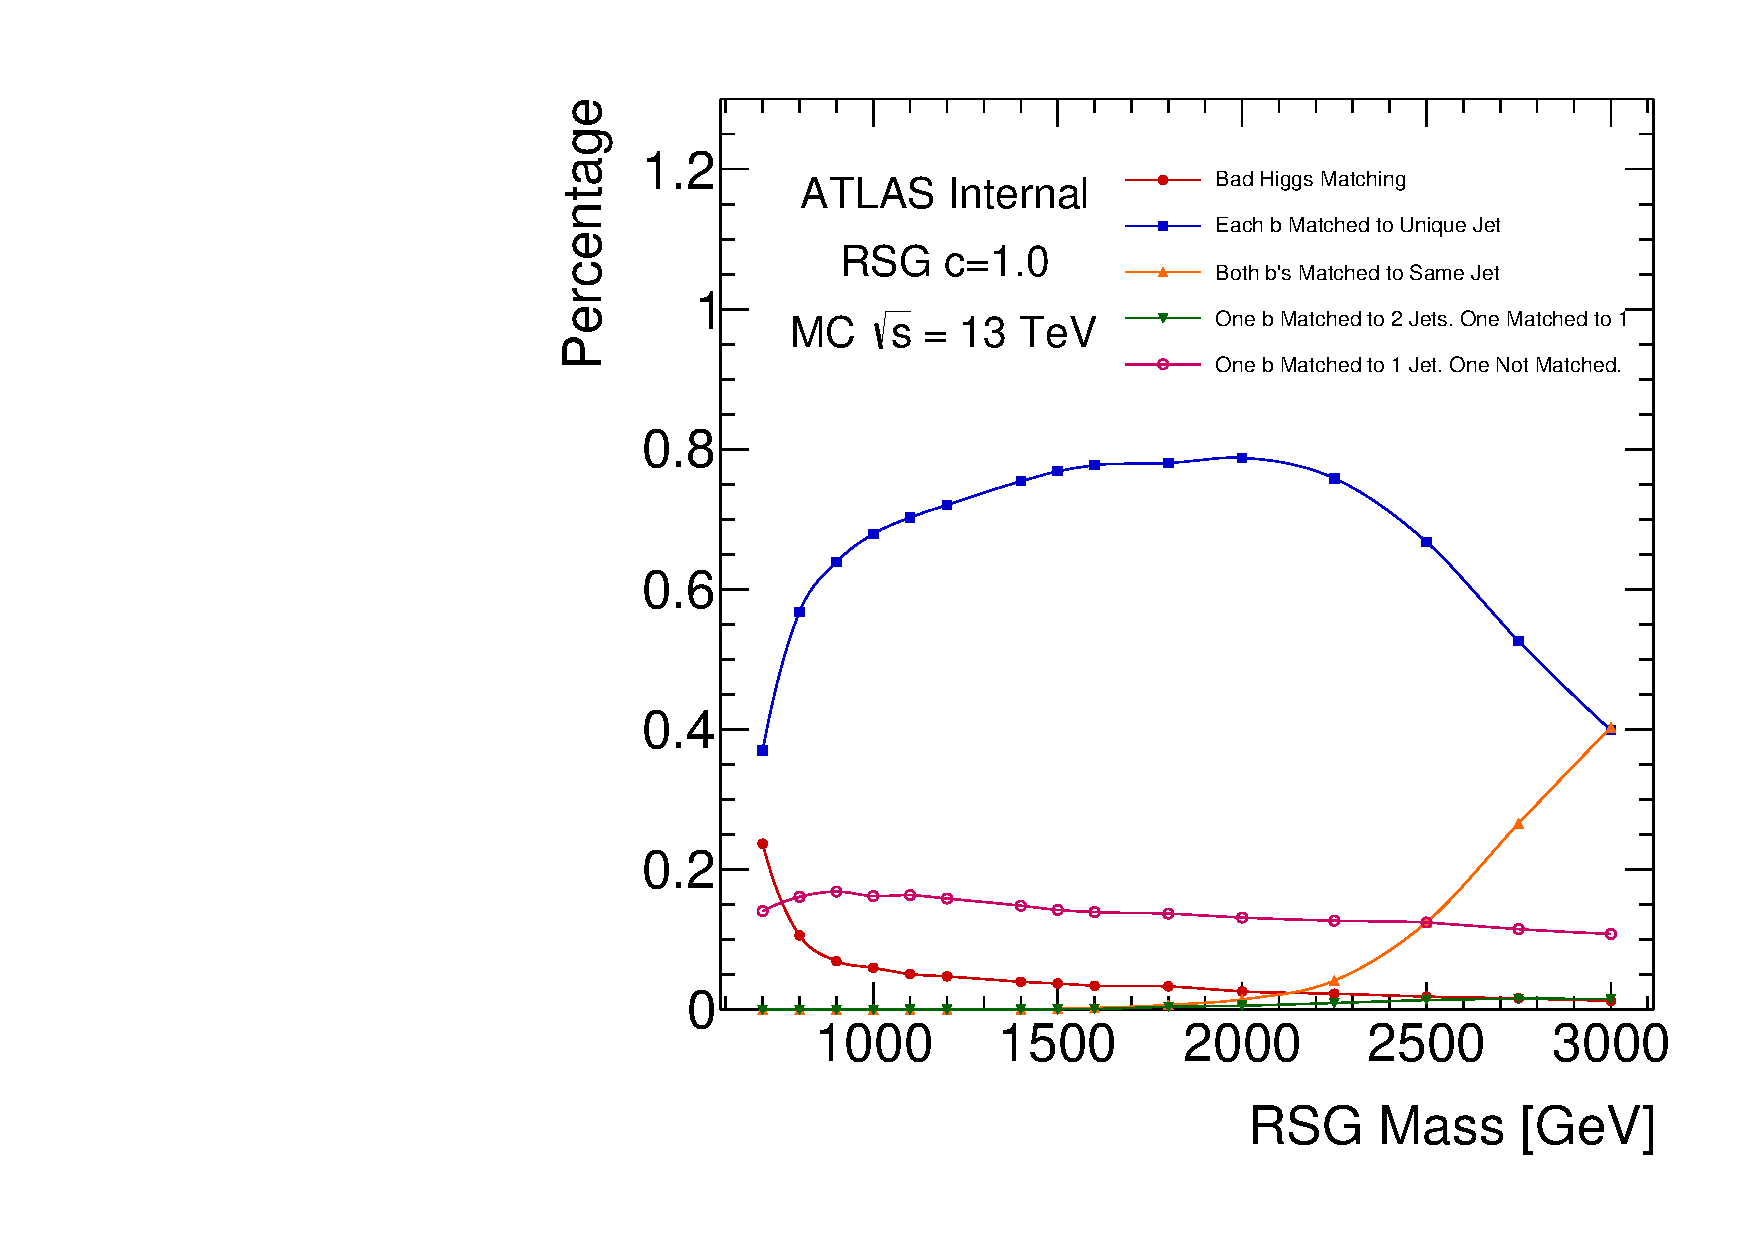
\includegraphics[width=0.45\textwidth,angle=-90]{figures/boosted/Truth/truth_b-matching-sublead.pdf}
\caption{Percentage of $\Delta R<0.2$ matching truth $b$'s to track jets (leading Higgs on the left, subleading Higgs on the right) for different \Grav~ mass. The cases listed in the legend are orthogonal to each other. The cases not listed on the legend (including when a truth $b$ is not contained in the large-\R jet) happen in total at most $1.6\%$ of the time for a given \Grav~ mass.}
\label{fig:truth-bmatch}
\end{center}
\end{figure}

\paragraph{}
A further muon correction accounts for energy loss due to leptonic $b$-hadron decays with a muon in the final state.
The muon-in-jet corrections are applied only after the fiducial large-\R jet requirements on \pt and $\eta$.
The muons are required have $\Delta R < 0.2$ with the $b$-tagged track jets within each large-\R jet. 
In case more than one muon is found within a track jet, only the muon with the smallest $\Delta R$ is considered. 
If two $b$-tagged track jets are found to have muons, both corrections are considered. 
The four-momenta of the matched muon is added to the large-\R jet four-momentum, with the muon calorimeter energy deposits subtracted. 
This correction is only applied to the calorimeter mass portion of the combined mass. 
The muon-in-jet correction improves the large-R jet mass resolution by approximately 5\%, and Figure~\ref{fig:boosted-muons-signal} shows the impact of this correction on the 1 \TeV~ \Grav.

\begin{figure*}
\begin{center}
  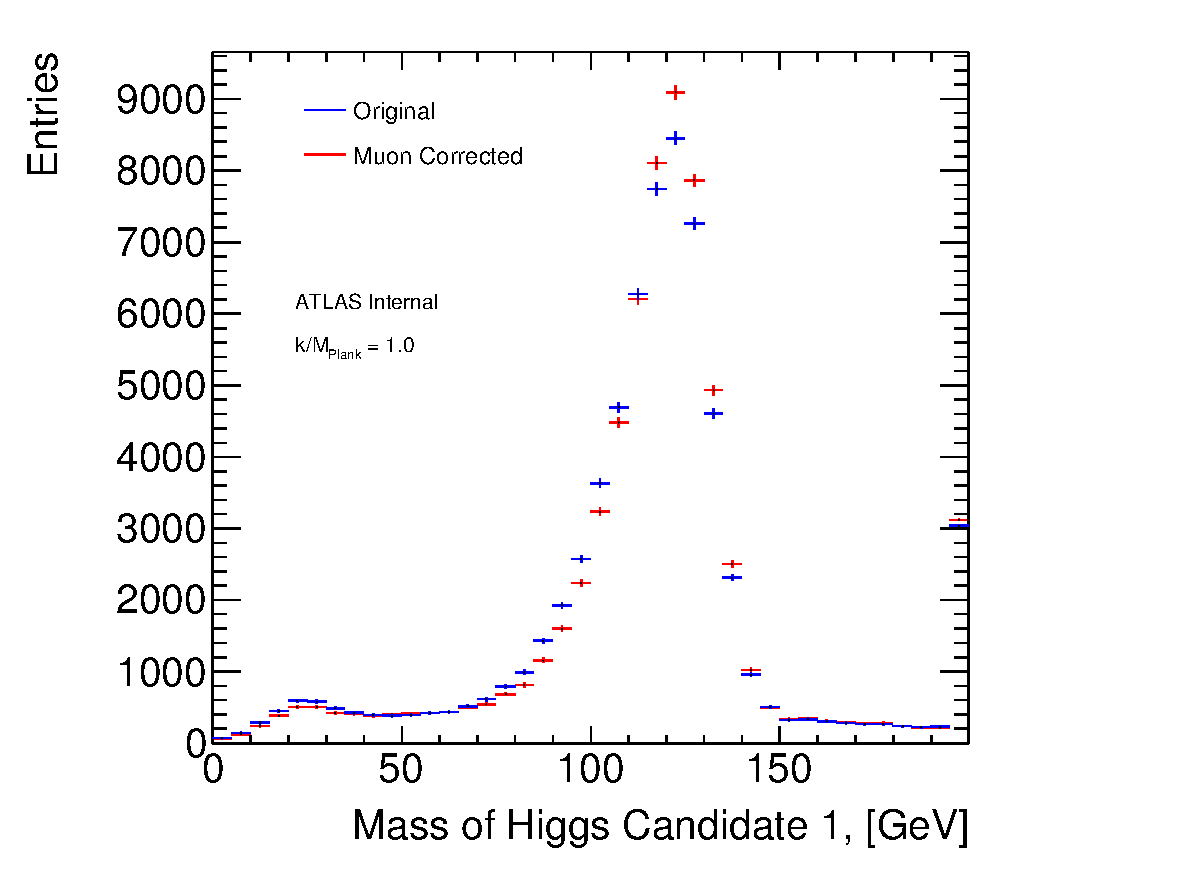
\includegraphics[width=0.48\textwidth]{figures/boosted/muons/h1_mass_dbl.pdf}
  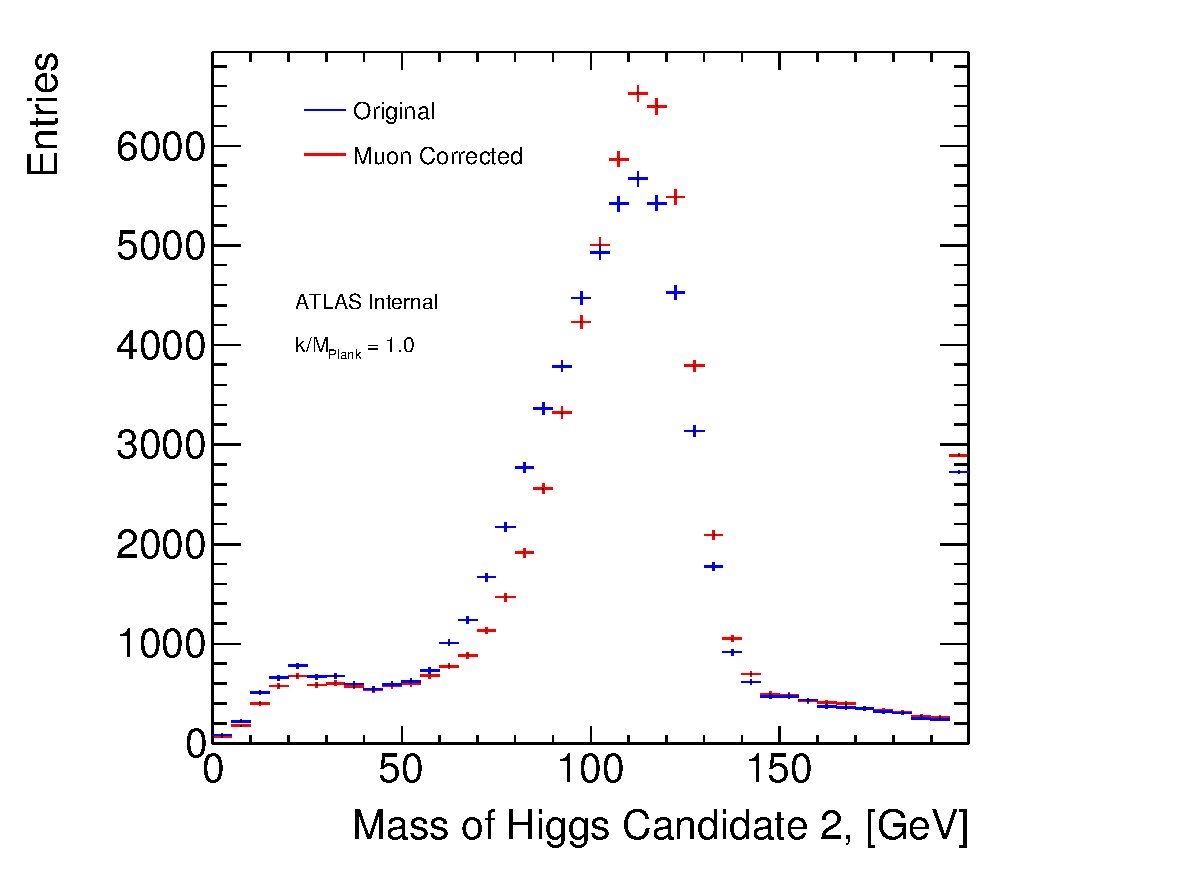
\includegraphics[width=0.48\textwidth]{figures/boosted/muons/h2_mass_dbl.pdf}
  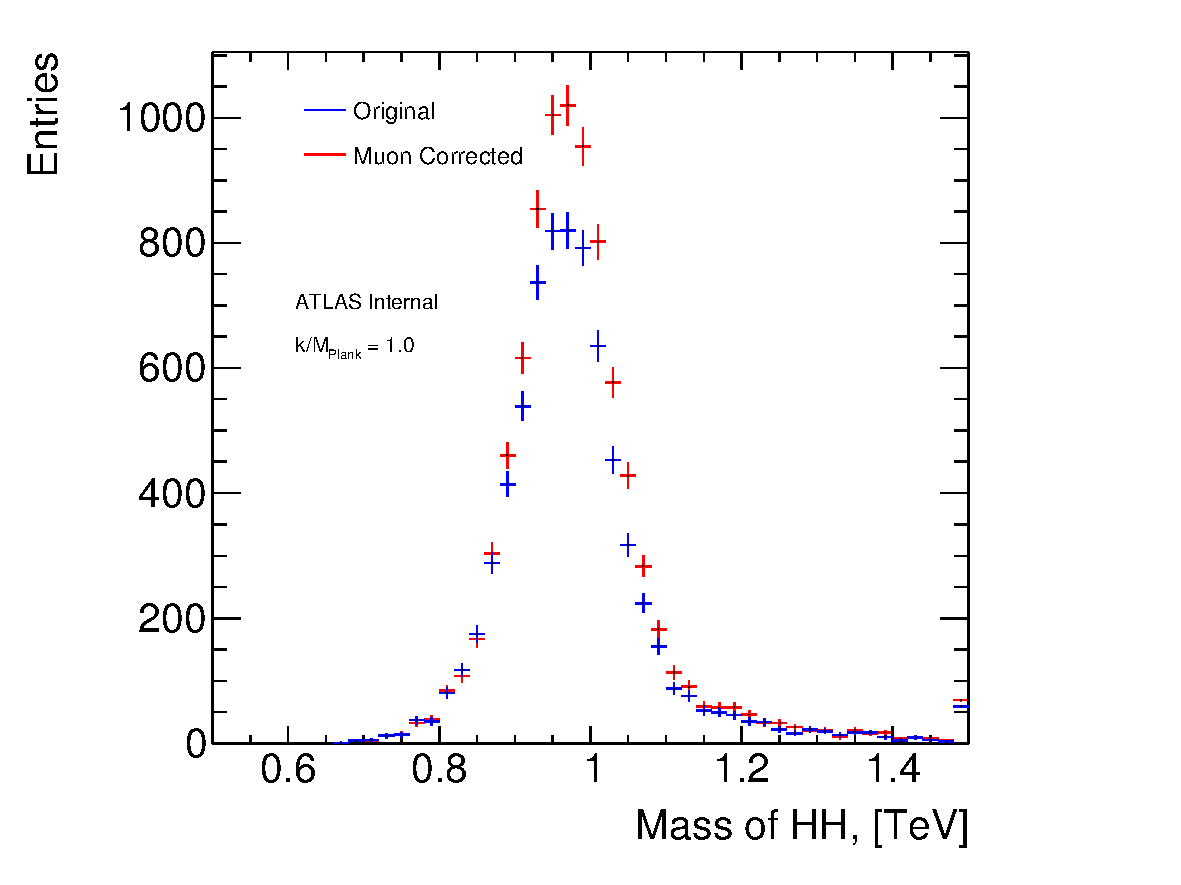
\includegraphics[width=0.48\textwidth]{figures/boosted/muons/hh_mass_dbl.pdf}
  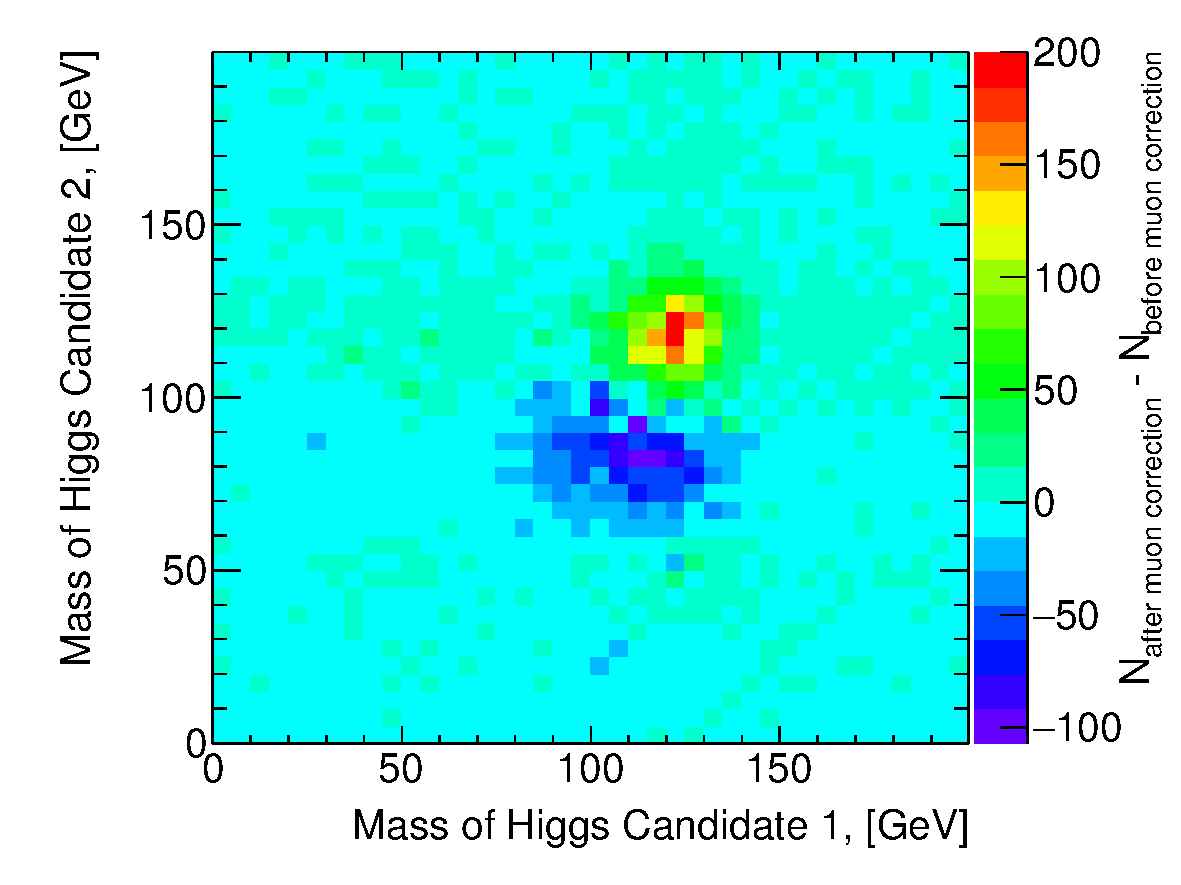
\includegraphics[width=0.48\textwidth]{figures/boosted/muons/h12_corr_mass.pdf}
  \caption{Kinematics of $1$ \TeV~ \Grav~ before and after muon-in-jet corrections. The reconstructed Higgs masses (top row, left for leading large-\R jet, right for subleading large-\R jet) are closer to $125$ \GeV after the correction, which improves the signal efficiency for the signal region selection by $\sim\!10\%$ (bottom row, left for $m_{JJ}$, right for event distribution differences on the leading-subleading large-\R jet mass plane.).}
  \label{fig:boosted-muons-signal}
\end{center}
\end{figure*}

\paragraph{}
Finally, the Higgs candidates (large-\R jets) are also required to have $|\Delta\eta| = |\eta_{\text{leadJ}} -\eta_{\text{sublJ}} |< 1.7$. 
This is because the spin 2 \Grav~ are produced mostly through s-channel, while the multijet events could also be produced through t-channels or u-channel. 
Figure ~\ref{fig:app-check-deta} shows the distribution for signal sample and data inclusive $b$-tag region $\Delta \eta_{JJ}$ distribution.
This cut is not entirely optimal for Scalar signals due to the different spin, yet it is fixed for both \Grav~ and Scalar selections.

\begin{figure*}
\begin{center}
  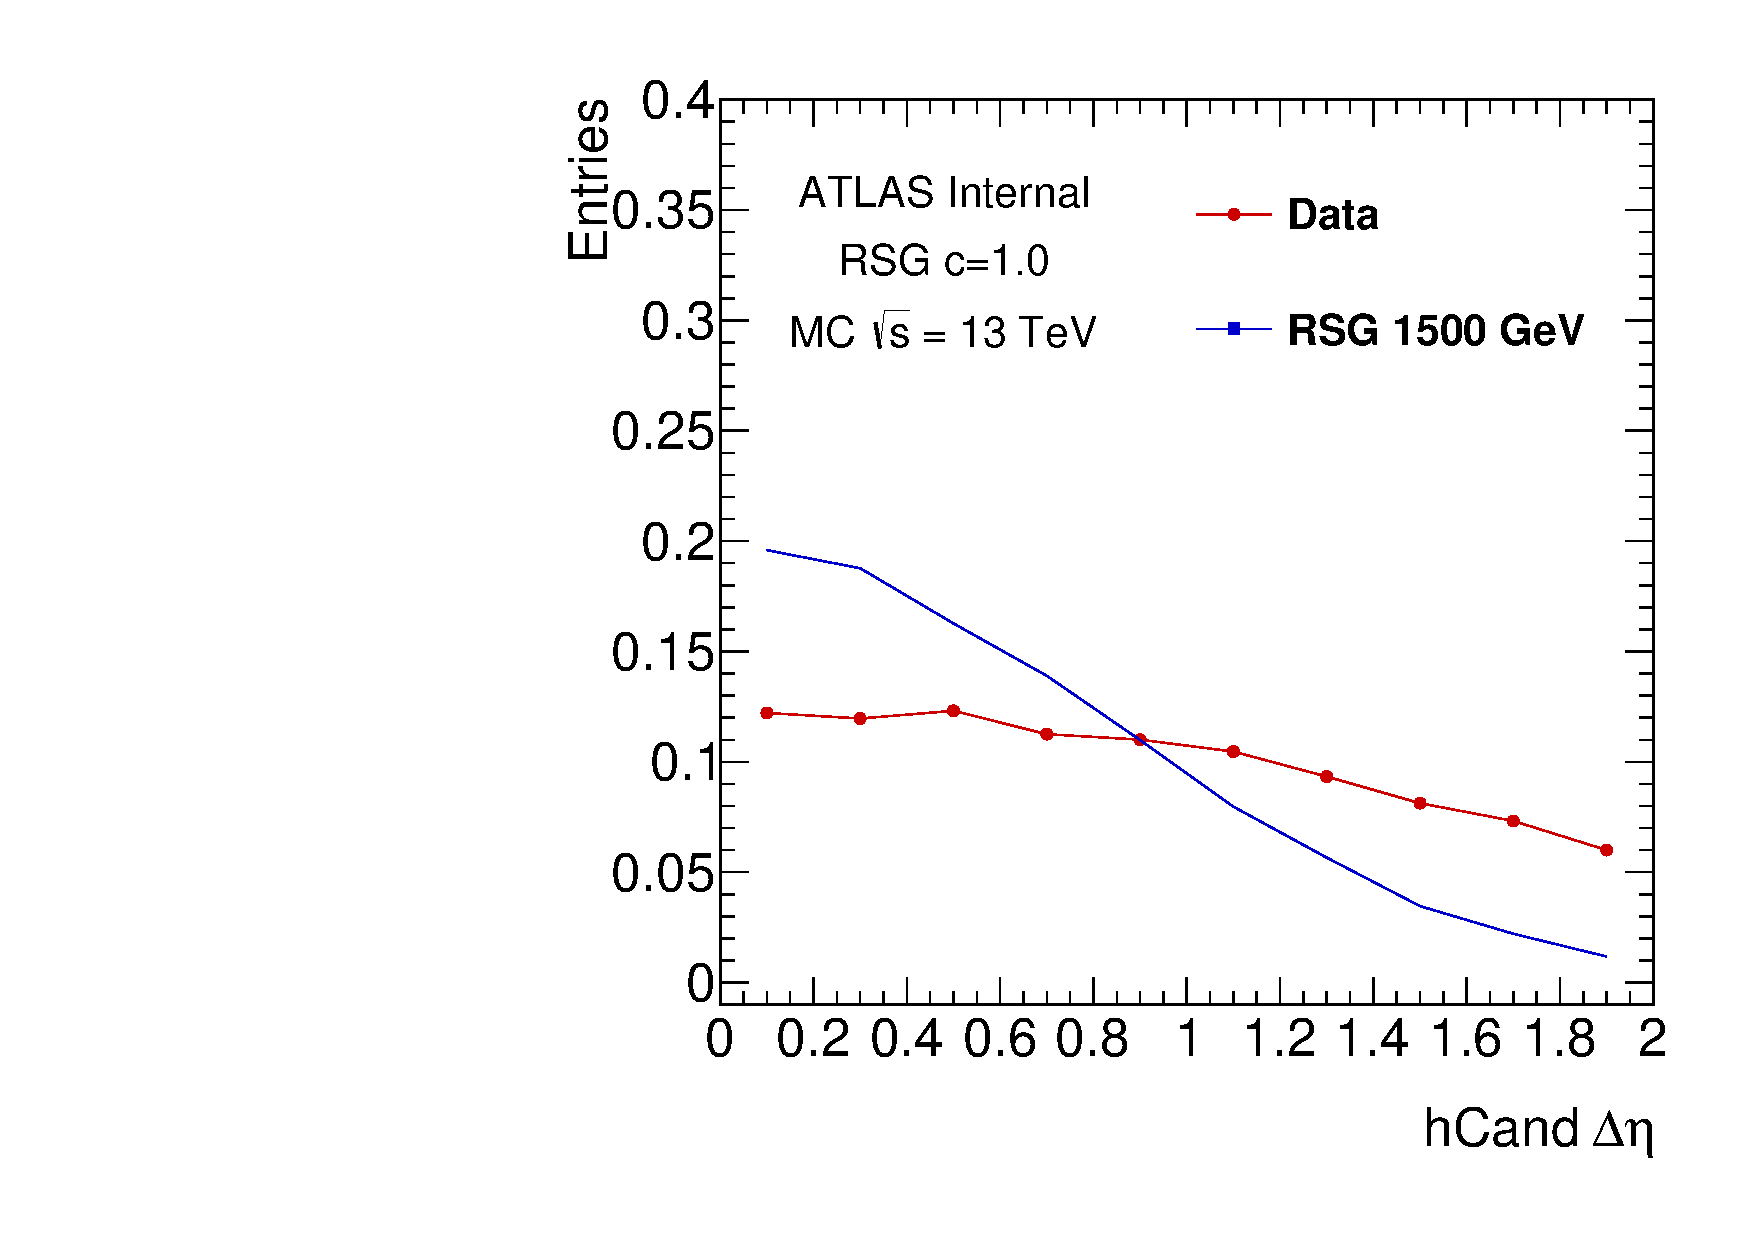
\includegraphics[width=0.45\textwidth,angle=-90]{figures/boosted/Other/AllTag_Signal_hCandDeta_F_c10-cb-no-deta-cut_truth_0.pdf}
  \caption{ After large-\R jet requirements, normalized $\Delta \eta_{JJ}$ distribution in $1.5$ \TeV \Grav~ and data, where the data consists of mostly multijet events (> 90$\%$). The background multijet event is flatter in $\Delta \eta_{JJ}$ distribution.}
\label{fig:app-check-deta}
\end{center}
\end{figure*}


%%%%%%%%%%%%%%%%%%%%%%%%%%%%%%%%%%%%%%%%%%%%%%%%%%%%%%%%%%%%%%%%%%%%%%%%%%%%%%%%%%%%%%%%%%
\section{Resolved Veto}
\label{sec:resollvedveto}

\paragraph{}
Sometimes one event can be reconstructed in both the resolved method as four small-\R jets and the boosted method as two large-\R jets with track jets. Figure~\ref{fig:obj_evt_display} shows an example event display of collision data recorded in 2015.

\begin{figure}[htbp!]
\centering
\captionsetup{justification=centering}
    \begin{subfigure}[b]{0.45\textwidth}
        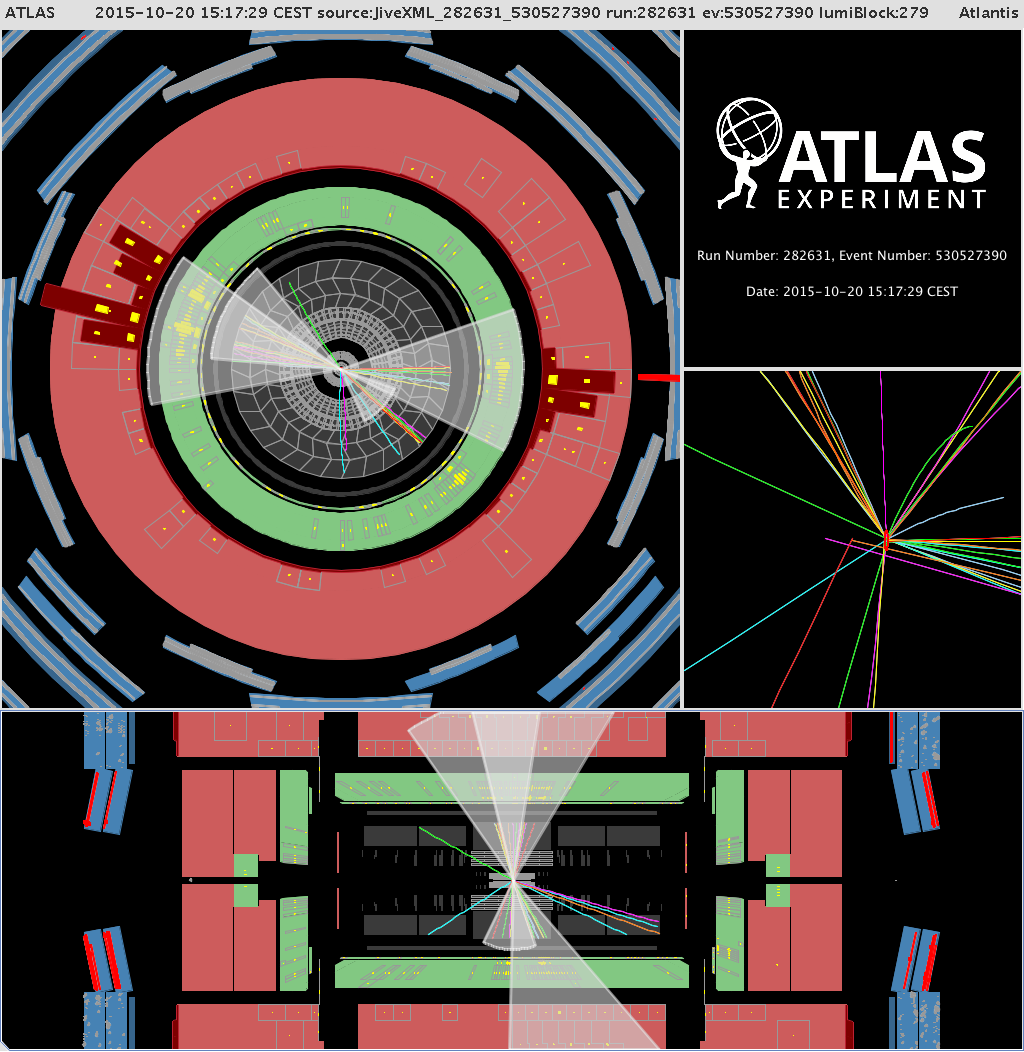
\includegraphics[width=\textwidth]{figures/object/JiveXML_282631_530527390-YX-RZ-YZ-EventInfo-2016-02-29-15-48-39}
        \caption{Resolved reconstruction.}
        \label{fig:obj_evt_display_resolved}
    \end{subfigure}
    \quad
    \begin{subfigure}[b]{0.45\textwidth}
        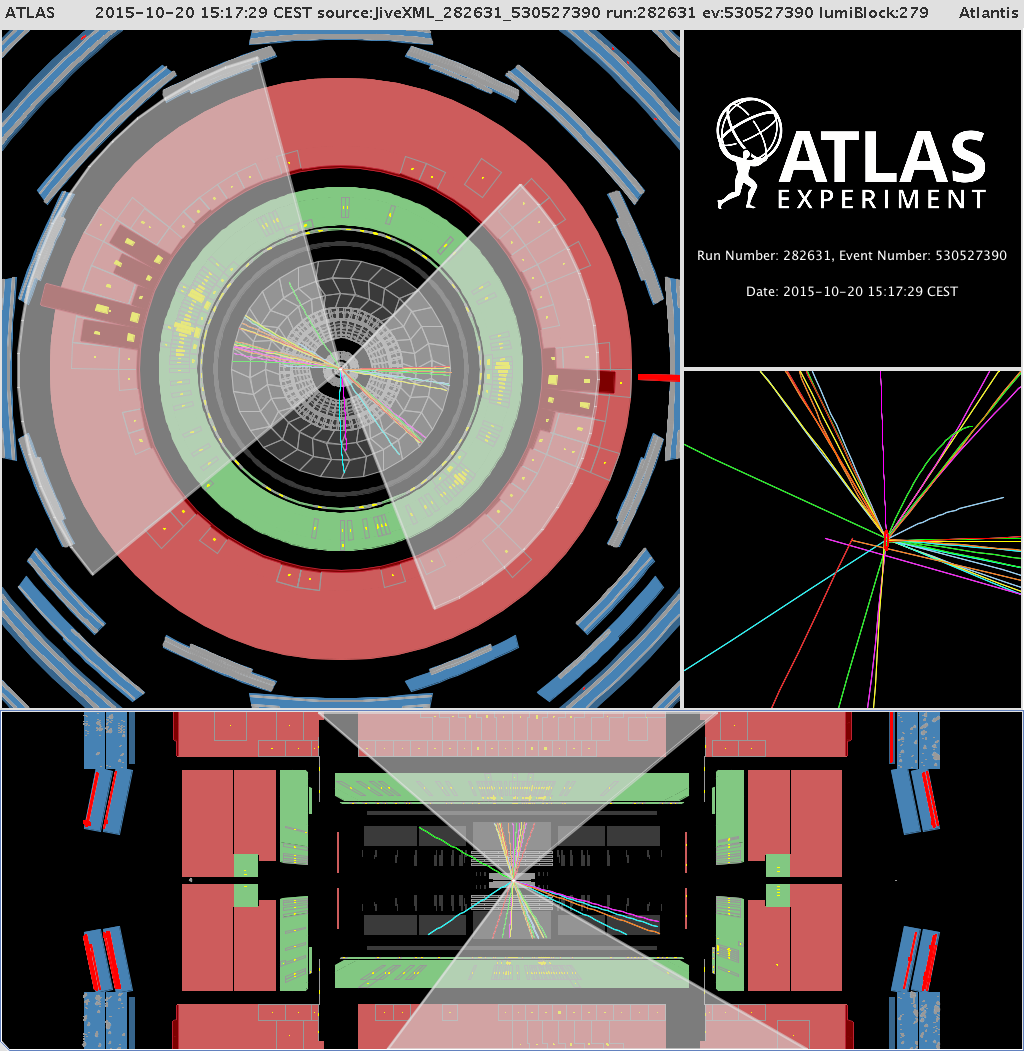
\includegraphics[width=\textwidth]{figures/object/JiveXML_282631_530527390-YX-RZ-YZ-EventInfo-2016-02-29-15-48-08}
        \caption{Boosted reconstruction.}
        \label{fig:obj_evt_display_boosted}
    \end{subfigure}
\caption{Event display of the same event using ~\ref{fig:obj_evt_display_resolved} resolved and ~\ref{fig:obj_evt_display_boosted} boosted topologies. The resolved reconstruction gives a $m_{4J}$ of $873$ \GeV~, and the boosted reconstruction gives $m_{2J}$ of $852$ \GeV. }
\label{fig:obj_evt_display}
\end{figure}

\paragraph{}
In order to avoid events being reconstructed by both the resolved and the boosted analysis, events that pass the resolved signal region selections are vetoed in the boosted analysis.
This is a political decision, and the effect of vetoing boosted event selection in the resolved analysis is never tested.
The gain is a full statistical combination of the resolved and boosted result.
For boosted analysis,  it hurts the sensitivity up to $1.5$ \TeV for resonance signals.
Hence it is necessary to introduce the resolved selection.

\paragraph{}
For resolved analysis, four small-\R jets with the highest $b$-tagging score are paired to construct two Higgs boson candidates.  
Each jet must have \pt $> 40$ \GeV~, $|\eta| < 2.5$, MV2c10 $> 0.8244$ (small-\R jet $70\%$ $b$-tagging working point). 
Pairings of jets into Higgs boson candidates are only accepted if they satisfy the following requirements, where \mfourj is expressed in \GeV:\\
if \mfourj  < 1250\,\GeV:
\begin{equation}
\frac{360\,\GeV}{\mfourj} - 0.5 < \DR_{jj}^{lead} < \frac{653\,\GeV}{\mfourj} + 0.475;\quad
\frac{235\,\GeV}{\mfourj} < \DR_{jj}^{subl}  < \frac{875\,\GeV}{\mfourj} + 0.35
\end{equation}
\quad if \mfourj  > 1250\,\GeV:
\begin{equation}
0< \DR_{jj}^{lead} < 1;\quad 0 < \DR_{jj}^{subl} < 1
\end{equation}
In these expressions, $\DR_{jj, \mathrm{lead}}$ is the angular distance between jets in the leading Higgs boson candidate and $\DR_{jj, \mathrm{subl}}$ for the sub-leading candidate. 
The leading Higgs boson candidate is defined to be the candidate with the highest scalar sum of jet \pt. 
This requirement efficiently rejects jet-pairings where one of the $b$-tagged jets is not consistent with that originating from a Higgs boson decay. 
The specific cut values in this and the following requirements were chosen to maximize the sensitivity to the signal.

\paragraph{}
Also, mass-dependent requirements are made on the leading Higgs boson candidate \pt, and the sub-leading Higgs boson \pt,:
\begin{equation}
p_T^{lead} > 0.5\mfourj - 105\,\GeV, \quad
p_T^{subl} > 0.33\mfourj - 75\,\GeV
\end{equation}
where \mfourj is again expressed in \GeV.

\paragraph{}
A further (\mfourj-independent) requirement is placed on the pseudorapidity difference between the two Higgs boson candidates, $\dEta < 1.5$, which rejects multijet events.
\begin{equation}
\dEta < 1.1 \quad \mathrm{if}\ \mfourj < 850\,\GeV , \quad
\dEta < 2\times10^{-3} \mfourj - 0.6 \quad \mathrm{if}\ \mfourj > 850\,\GeV
\end{equation}

\paragraph{}
Events that have multiple Higgs boson candidates satisfying these requirements (which happens often when $\mfourj < 500\,\GeV$) necessitate an algorithm to choose the correct pairs. 
In the absence of energy loss through semi-leptonic decays, the optimal choice would be the combination most consistent with the decays of two particles of equal mass.
To account for energy loss, the requirement of equal masses is modified. 
The distance, \Dhh, of the pairing's leading and subleading Higgs boson candidate masses, $\left(\leadm, \sublm\right)$ from the line connecting $\left(0\,\GeV, 0\,\GeV\right)$ and $\left(120\,\GeV, 110\,\GeV\right)$ is computed, and the pairing with the smallest value of \Dhh~ is chosen.
The values of 120\,\GeV\, and 110\,\GeV\, are chosen because they correspond to the median values of the narrowest intervals that contain 90\% of the signal in simulations.%the centre of the signal region in \leadm and \sublm respectively,
\Dhh~ can be expressed as follows:
\begin{equation}
D_{hh} = \frac{\left|\leadm - \frac{120}{110}\sublm\right|}{\sqrt{1+\left(\frac{110}{120}\right)^{2}}}.
\end{equation}

\paragraph{}
A requirement on the Higgs boson candidates' masses is used to define the resolved signal region:
\begin{equation}
X_{hh-resolved} = \sqrt{\left(\frac{\mlead - 120\,\GeV}{0.1\mlead}\right)^2 + \left(\frac{\msubl - 110\,\GeV}{0.1\msubl}\right)^2} < 1.6,
\label{eqn:resolvedXhh}
\end{equation}
where the 0.1\mtwoj terms represent the widths of the leading and sub-leading Higgs boson candidate mass distributions, derived from simulation. The signal region is shown as the inner region of Figure~\ref{fig:resolvedRegions}. In summary, for any event can make a Higgs candidate through the Dhh minimization and passing through the resolved signal region $X_{hh-resolved}$ cut, it is rejected in the boosted selection.

%For more detail, please see the resolved signal region definition. 
%For the impact on the boosted analysis, see Appendix ~\ref{sec:app-optimization-resveto}.

%%%%%%%%%%%%%%%%%%%%%%%%%%%%%%%%%%%%%%%%%%%%%%%%%%%%%%%%%%%%%%%%%%%%%%%%%%%%%%%%%%%%%%%%%%

\section{2D Higgs Mass Cut}

\begin{figure*}[htbp!]
\begin{center}
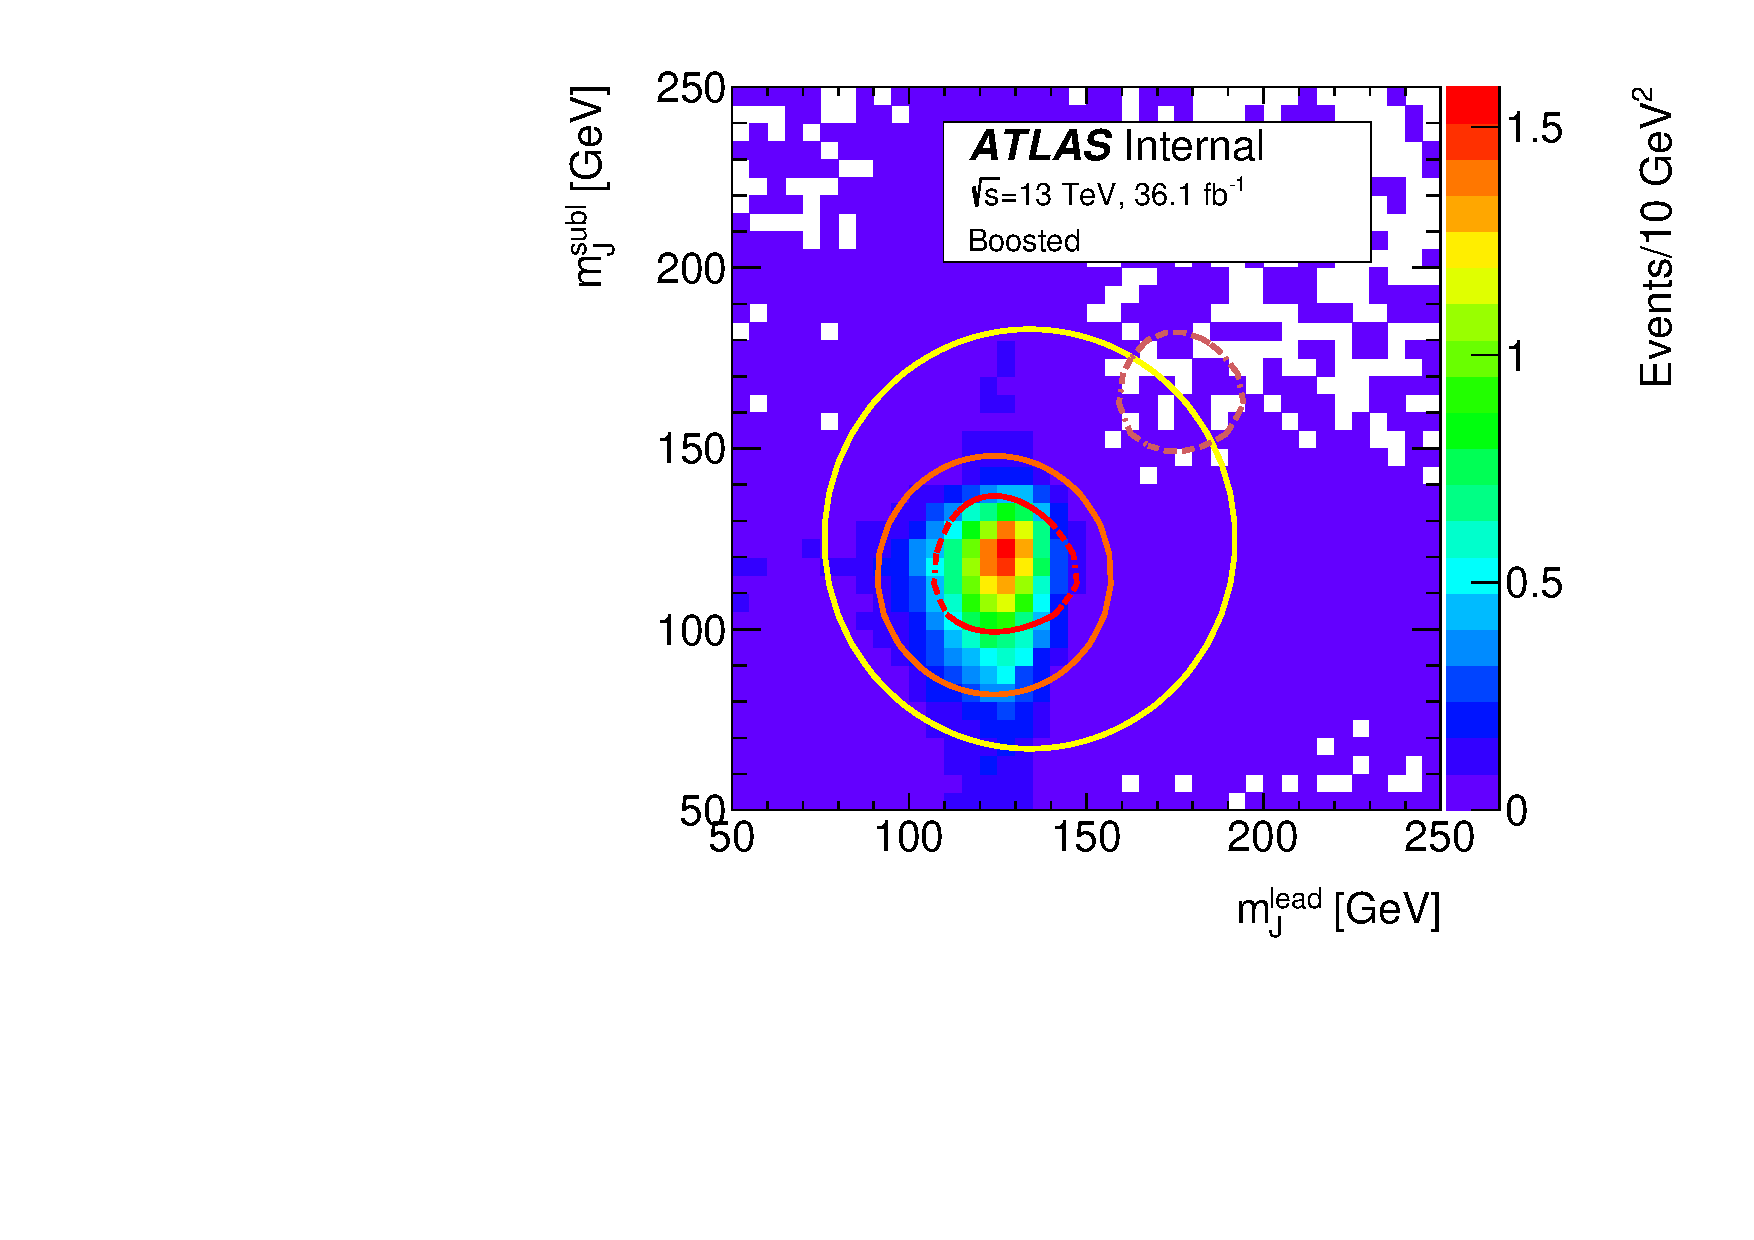
\includegraphics[width=0.35\textwidth,angle=-90]{figures/boosted/Truth/Sig_1200_AllTag_Incl_mH0H1.pdf}
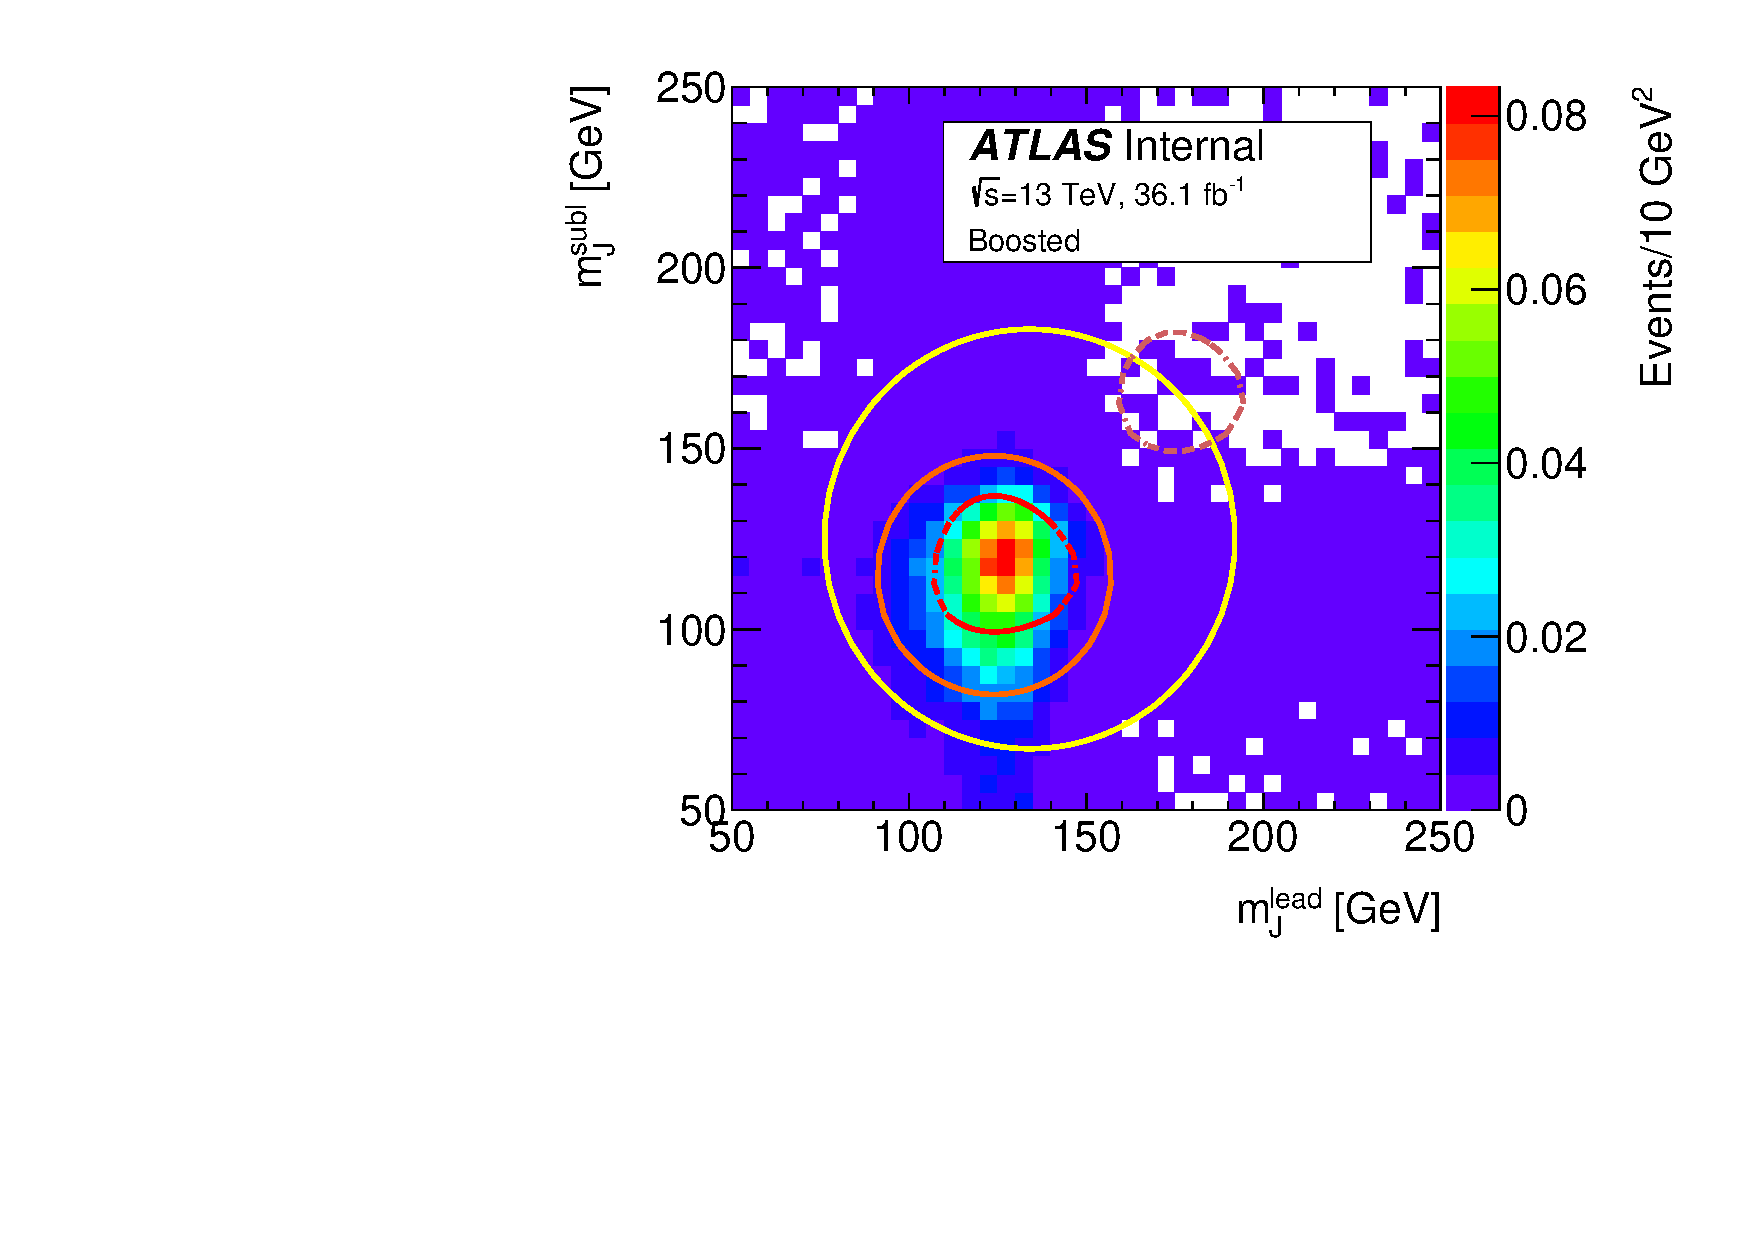
\includegraphics[width=0.35\textwidth,angle=-90]{figures/boosted/Truth/Sig_2000_AllTag_Incl_mH0H1.pdf}
\caption{For RSG $c=1.0$ samples, number of events as a function of leading Higgs candidate mass and subleading Higgs candidate mass, for $1.2$ \TeV~(left) signal and $2$ \TeV~(right) signal samples. The red dotted line in the center correspond to the signal region, passing $X_{hh} < 1.6$.}
\label{fig:evt-signal-mhh}
\end{center}
\end{figure*}

\paragraph{}
To separate di-Higgs decays from background productions like QCD multi-jets and top, requirements on the leading and subleading large-\R jet masses are imposed.
The signal region is defined using the expression~\ref{eq:boosted_XhhDef}:
\begin{equation}
\label{eq:boosted_XhhDef}
X_{hh} = \sqrt{\left(\frac{m^{\rm lead}_{\rm J} - \text{124 GeV}}{0.1 \left(m^{\rm lead}_{\rm J}\right)}\right)^2 + \left(\frac{m^{\rm subl}_{\rm J}- \text{115 GeV}}{0.1 \left(m^{\rm subl}_{\rm J}\right)}\right)^2}
\end{equation}

\paragraph{}
The denominator of each term in \Xhh~ can be interpreted as a resolution on the reconstructed mass of $10\%$ for the leading and subleading jets, hence \Xhh~ can be interpreted as a $\chi^2$ compatibility with the di-Higgs hypothesis.
The subleading jet mass value of $115$ \GeV~ is chosen after investigating the signal jet masses in MC. 
The subleading large-\R jet typically has a reconstructed mass which is biased downward. 
This is partly due to the ordering of the large-\R jets in \pt, which makes the subleading jet towards lower energy. 
The energy losses from neutrinos in leptonic $b$ decays, cracks in the calorimeter, and other effects also contributes. 
The signal region requires $X_{hh} < 1.6$. 
This cut gives nearly optimal performance. 
A more optimal signal region definition, using asymmetric signal jet mass resolution and a momentum dependent cut accounting for the higher mass resolution of lager \pt~ jets, can improve the overall sensitivity by $2-8\%$.
Since the gain in sensitivity is small, the signal region is kept to be consistent with the $X_{hh-resolved}$. Figure ~\ref{fig:evt-signal-mhh} shows the \Grav~ MC \mlead-\msubl 2D distribution.

%The denominator of each term in the definition can be interpreted as a resolution on the reconstructed mass of $8.5\%$ for the leading jet and $12\%$ for the subleading jet, hence $X_{hh}$ can be interpreted as a $\chi^2$ compatibility with the $hh$ hypothesis. Similarly to the resolved analysis, these $\sigma \left(m_{\rm J}\right)$ are only a rough approximation to the true resolution, but the $X_{hh}$ requirement gives nearly optimal performance. 
%The last substraction for high $p_\text{T}$ cases is because of the higher mass resolution of high mass signal samples. This effectively increases the size of $X_{hh}$ to 1.8 for a 3 TeV signal.

\section{Number of $b$-tagging requirement}
\paragraph{}
Passing basic object selection and \Xhh~ cut, the signal region selection is defined by further requiring multiple $b$-tags which are consistent with the di-Higgs decay. 
The presence of two \hbb~ decays in the final state naturally suggests requiring 4 track jets passing $b$-tagging requirements, and this is defined as the  $4b$ selection.

\paragraph{}
The $4b$ requirement has an overall efficiency of roughly $\epsilon^4$, where $\epsilon$ is the $b$-tagging efficiency chosen to be $70\%$.
This means an overall $0.7^4 \sim 0.24$ probability, but having one actual $b$-jet failling while the other three pass has probability $3 \times 0.7^3 \times (1-0.7) \sim 0.31$.
Therefore, a $3b$ selection is also introduced to recover the signal efficiency. 
An event with $3b$-tags must have at least $3b$-tagged track jets, but can have any number of additional un-tagged track jets.
In $4b$ and $3b$, each Higgs candidate can have at most two $b$-tagged track jets, hence $\geq 3b$-tagged track jets cannot be in the same large-\R jet.

\paragraph{}
At the highest resonance mass, the Lorentz boost of the Higgs boson can be large enough to collimate the daughter $b$-quarks below the distance scale resolvable by the track jets ($R=0.2$). A third signal region is denoted by two-tag-split or simply $2bs$.
It requires exactly one $b$-tagged track jet is found in each Higgs candidate, plus an arbitrary number of track jets that must fail the $b$-tag.

\paragraph{}
$4b$, $3b$, and $2bs$ regions are chosen as three signal regions, also referred to as $n$-$b$tag regions.
The other $b$-tagging situations, also referred to as lower-$b$tag regions, are also sorted and studied.
$2b$ region is defined as one large-\R jet has two $b$-tagged track jets, and the other large-\R jet has no $b$-tagged track jet. 
$1b$ region is defined as one large-\R jet has one and only one $b$-tagged track jets, and the other large-\R jet has no $b$-tagged track jet. 
$0b$ region is defined as both large-\R jets have no $b$-tagged track jet. 
They all have relatively small signal acceptance. 

\paragraph{}
The MC events passing all signal region selections are sorted into different $b$-tagging categories. This is shown in Figure~\ref{fig:boosted-nbjet-signal-efficiency}. 
For masses above 2.5 TeV, the $2bs$ region (where each large-\R jet has exactly one $b$-tagged track jet) significantly improves the acceptance.
\begin{figure*}
\begin{center}
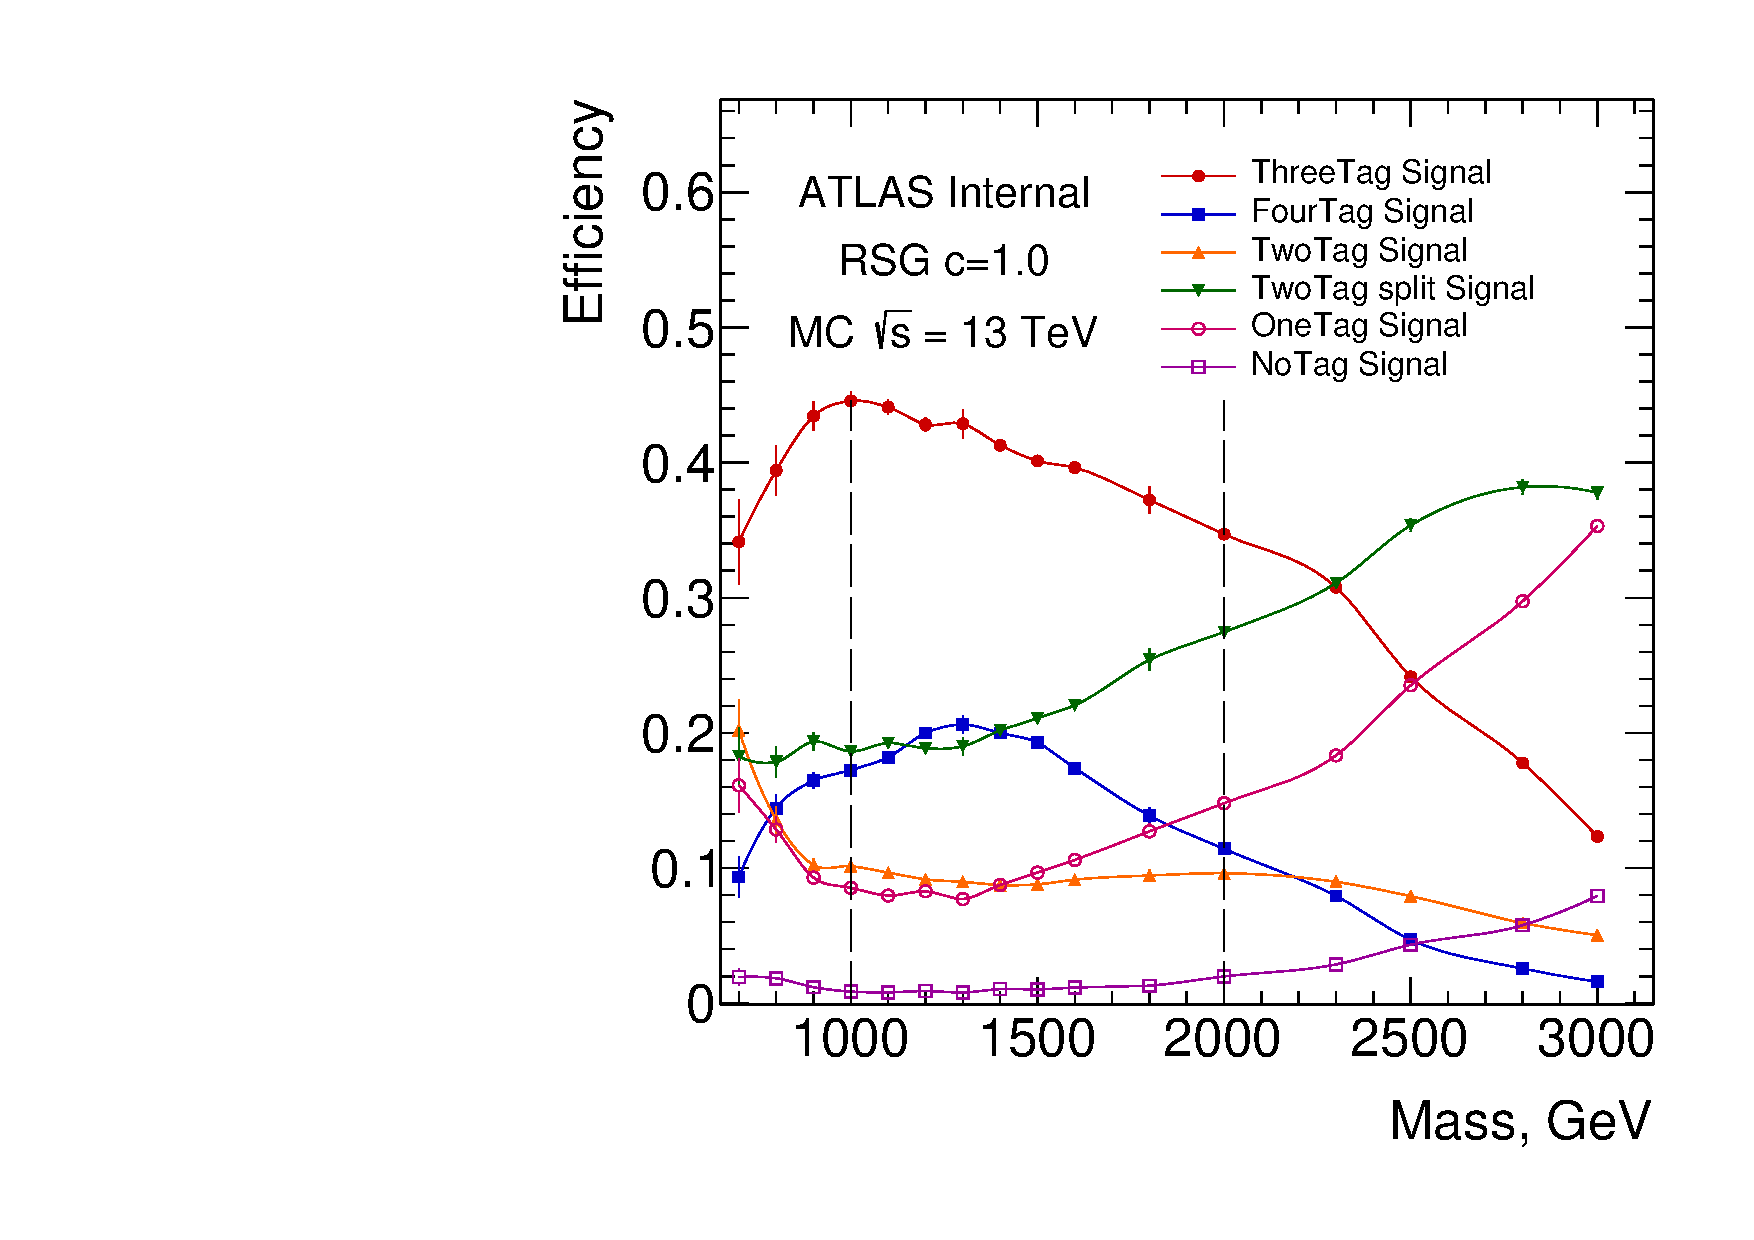
\includegraphics[width=0.48\textwidth,angle=-90]{figures/boosted/SigEff/region_lst_Moriond_Efficiency_AllTag_Signal.pdf}
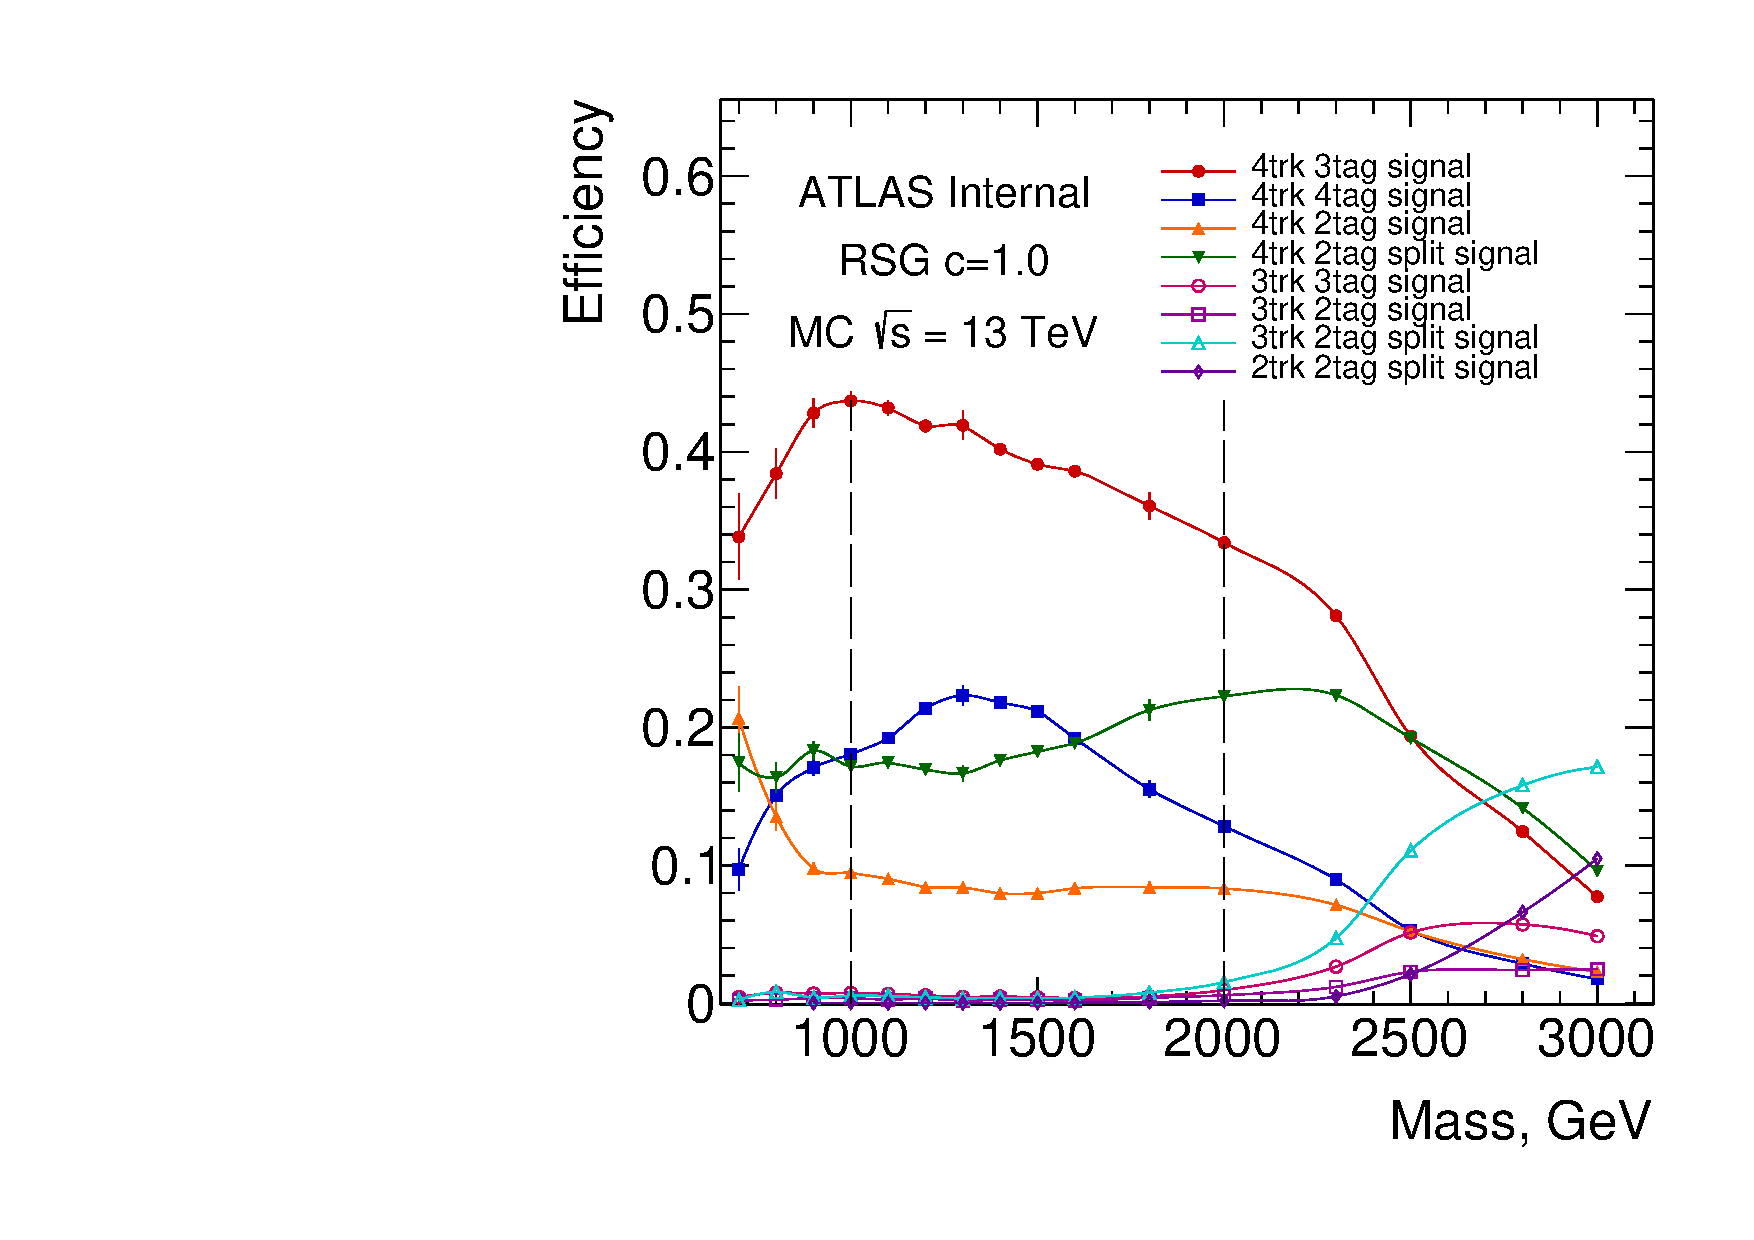
\includegraphics[width=0.48\textwidth,angle=-90]{figures/boosted/SigEff/detail_lst_Moriond_Efficiency_AllTag_Signal.pdf}
  \caption{Signal fraction in different $b$-tag categories (left) and detailed fraction in different number of track jet and $b$-tag categories (right) as a function of signal resonance mass hypothesis for selection cuts. The efficiencies are relative to the total number of events passing the 2D mass cut.}
  \label{fig:boosted-nbjet-signal-efficiency}
\end{center}
\end{figure*}



%%%%%%%%%%%%%%%%%%%%%%%%%%%%%%%%%%%%%%%%%%%%%%%%%%%%%%%%%%%%%%%%%%%%%%%%%%%%%%%%%%%%%%%%%%
\section{Signal efficiency and cutflow}
\paragraph{}
Acceptance means purely geometric fiducial volume of the detector. Efficiency refers to purely detector effectiveness in finding objects.
The signal efficiency as a function of \Grav~ resonance mass is shown in Figure~\ref{fig:boosted-selection-efficiency}, both for the absolute signal efficiency and for the efficiency relative to the previous cut in the selection.
Above a mass of $\sim\!1$ \TeV, the reconstruction of high momentum large-\R jets with small $\Delta\eta$ is efficient. 
Across the mass range considered, the signal jet masses requirement ($X_\text{hh}$) and $b$-tagging requirements are $\mathcal{O}(20\%)$ efficient relative to the previous cuts.

\begin{figure*}
\begin{center}
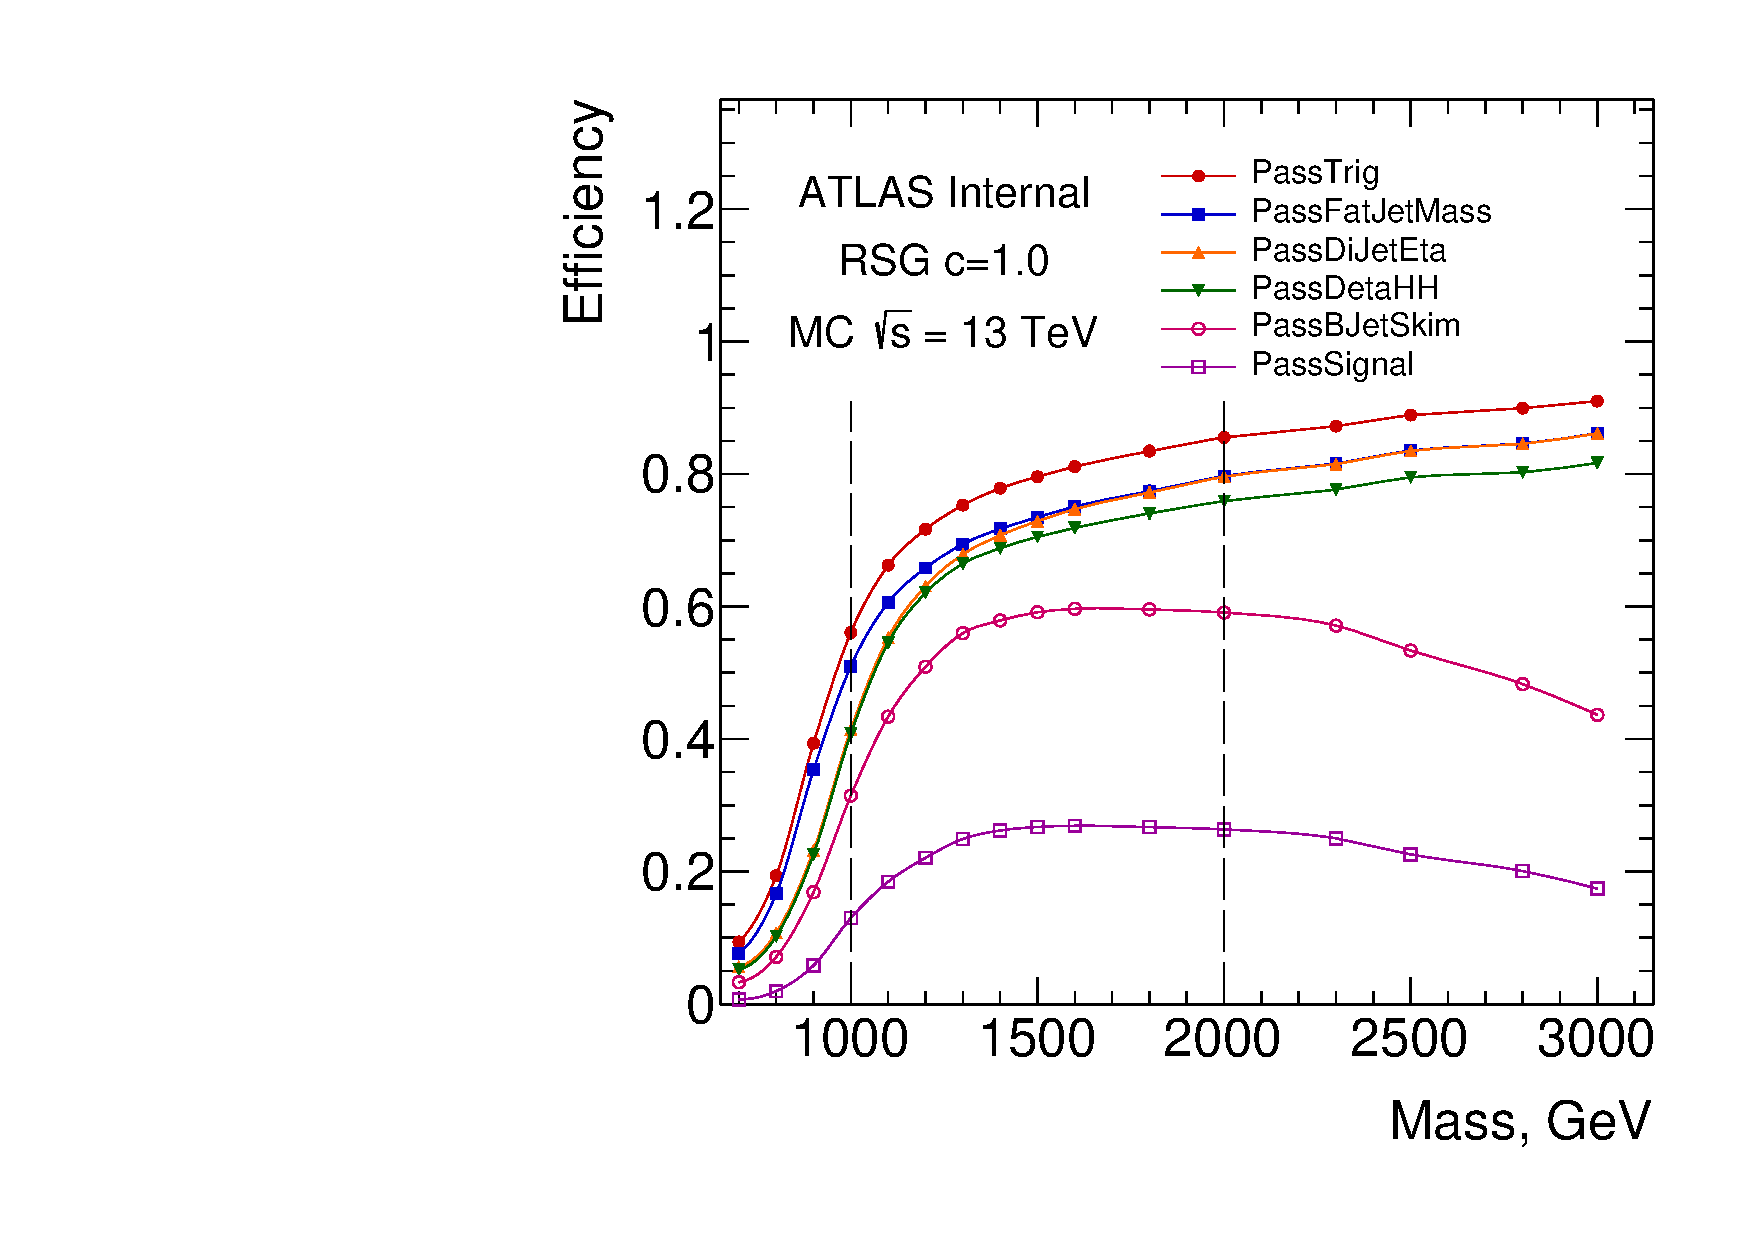
\includegraphics[width=0.48\textwidth,angle=-90]{figures/boosted/SigEff/evtsel_Moriond_Efficiency_PreSel.pdf}
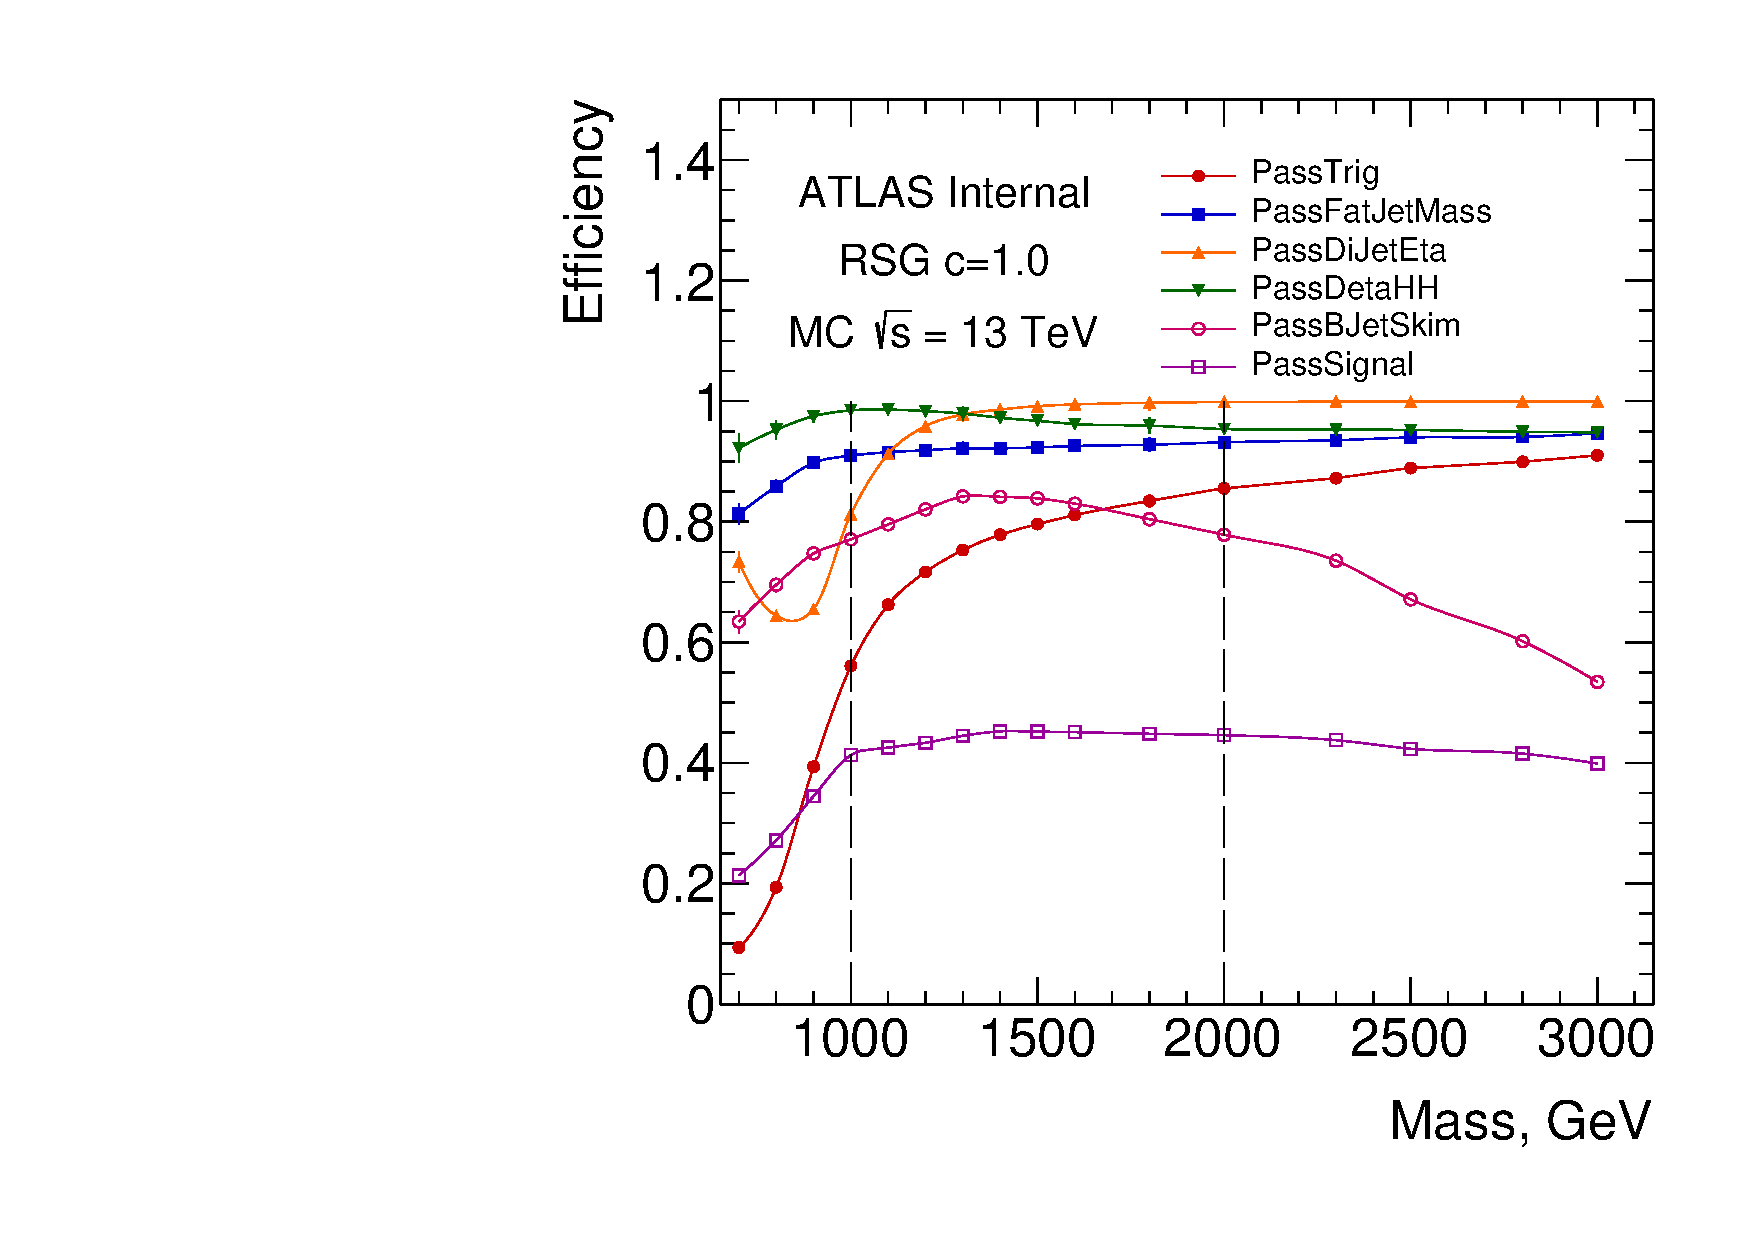
\includegraphics[width=0.48\textwidth,angle=-90]{figures/boosted/SigEff/evtsel_Moriond_Efficiency_PreSel_rel.pdf}
  \caption{Absolute (left) and relative (right) signal efficiency as a function of RSG c=1.0 signal resonance mass hypothesis for selection cuts. The relative efficiency is defined from the previous cut, where the order of cuts is given by the legend. PassTrig means the event passes the trigger selection; PassDiJetPt means the event passes the leading and sub-leading jet \pt cuts; PassDiJetEta means the event passes the leading and sub-leading jet $\eta$ cuts; PassDetaH means the events passes the $|\Delta \eta| < 1.7$ cut; PassBJetSkim means the event contains at least two $b$-tagged track jets, inclusive of $2b$, $2bs$, $3b$ and $4b$ configurations; PassSignal means the event passes the signal region cut $X_{hh} < 1.6$.}
  \label{fig:boosted-selection-efficiency}
\end{center}
\end{figure*}

\paragraph{}
The selection efficiency at various stages for \Grav with $c=1.0$, \Grav with $c=2.0$, and Heavy Scalar signal samples of all mass points can be found in Table~\ref{boosted-eff-RSG_c10}, ~\ref{boosted-eff-RSG_c20} and ~\ref{boosted-eff-2HDM}.


% \begin{figure*}
% \begin{center}
% \subfloat[]{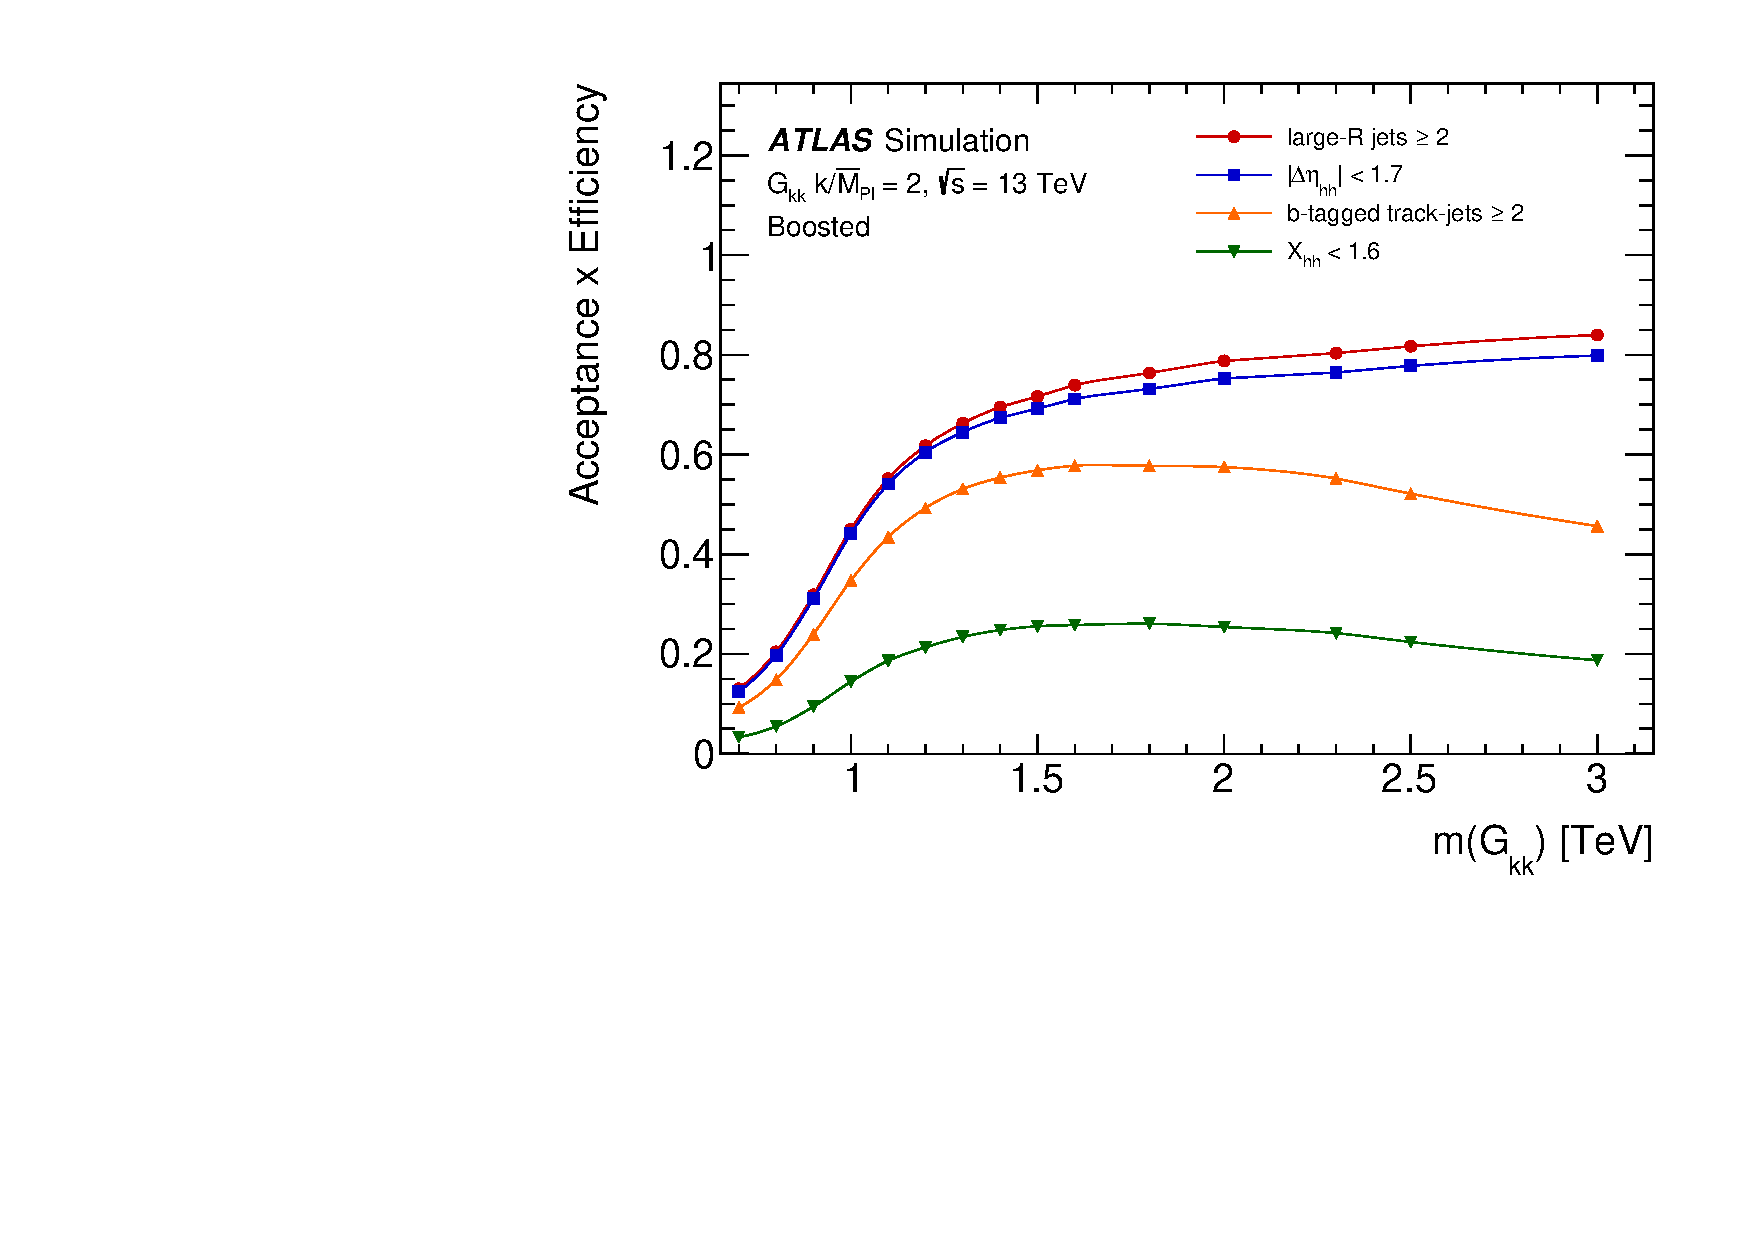
\includegraphics[width=0.48\textwidth,angle=-90]{figures/boosted/SigEff/G_hh_c20_evtsel_Moriond_bkg_9_Efficiency_PreSel.pdf}
% \subfloat[]{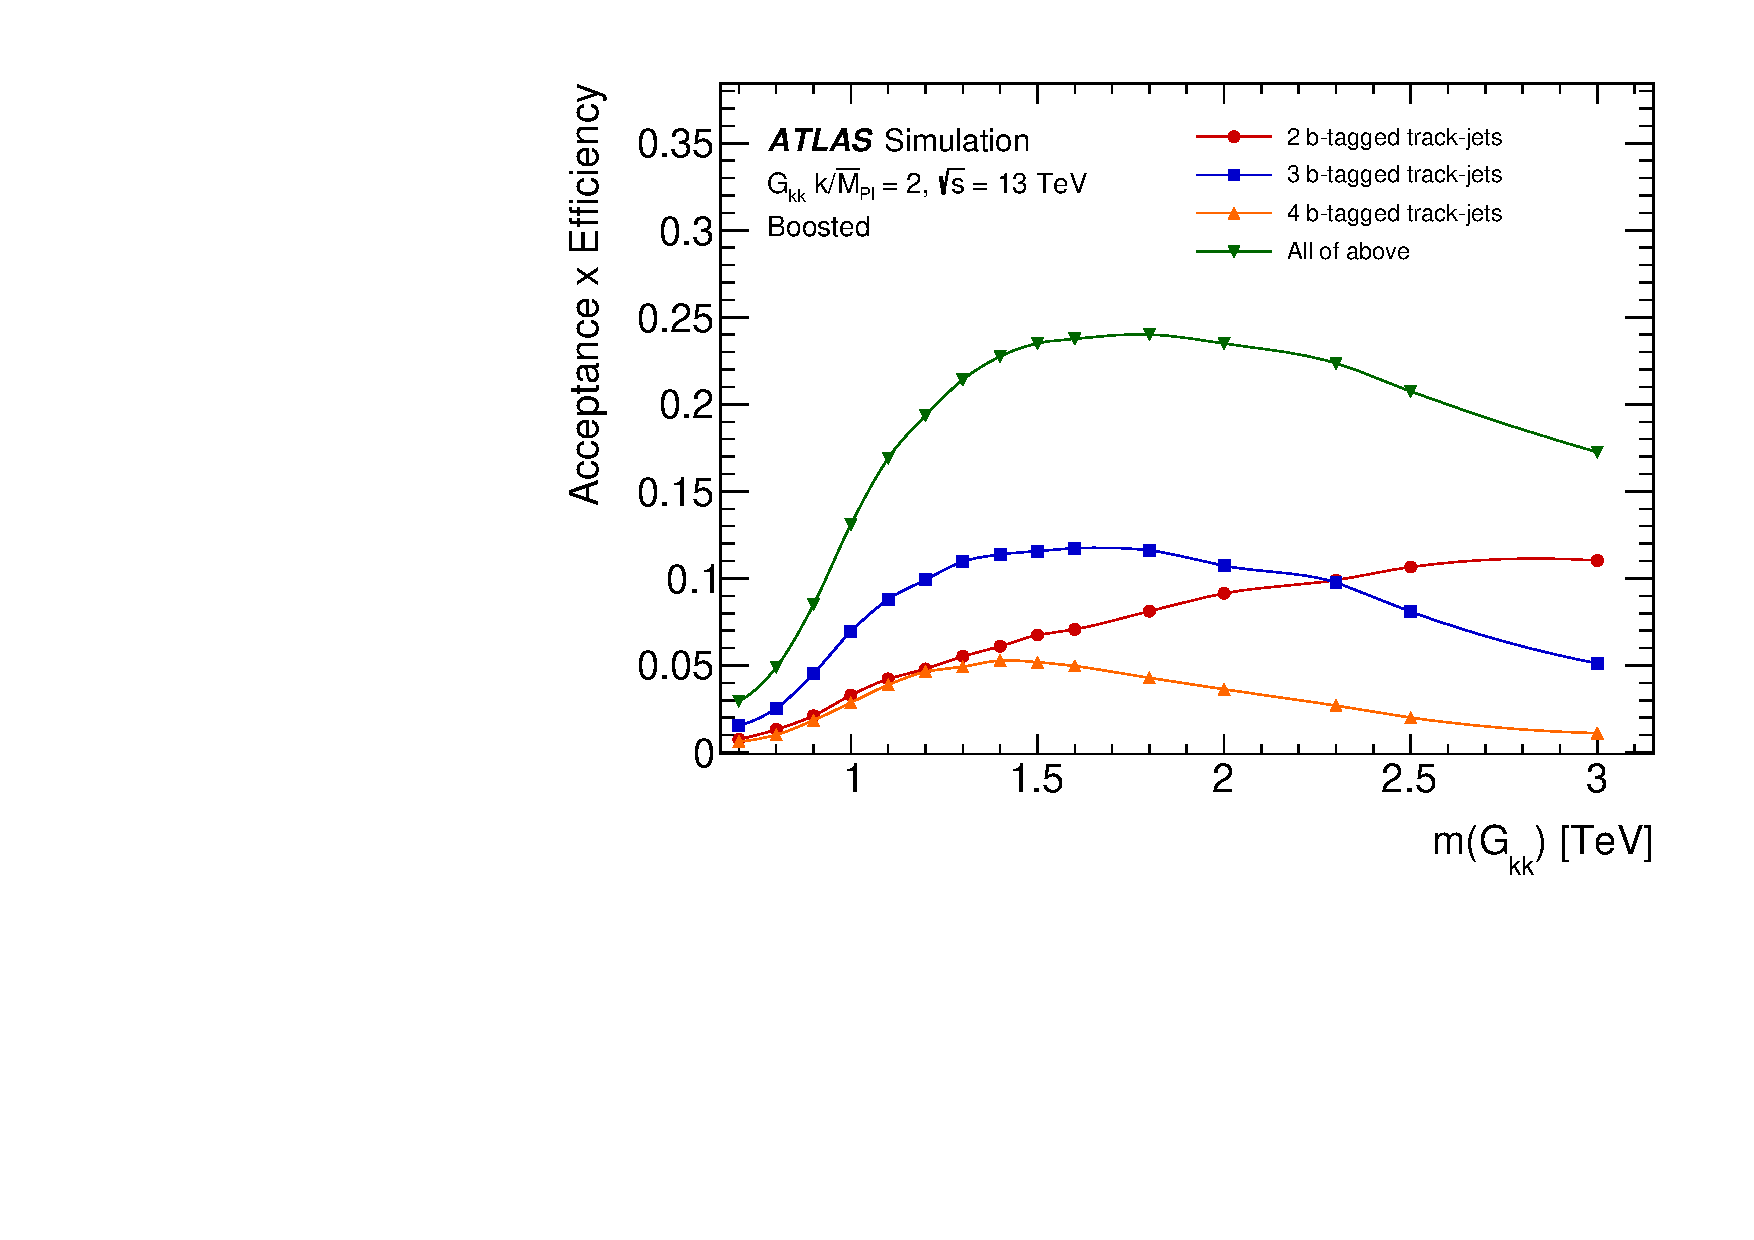
\includegraphics[width=0.48\textwidth,angle=-90]{figures/boosted/SigEff/G_hh_c20_region_lst_Moriond_bkg_9_Efficiency_PreSel.pdf}
% \caption{(a) The selection acceptance times efficiency of the boosted analysis at each stage of the event selection as a function of the generated graviton mass for $\kMPl = 2$. The trigger efficiency is approximately 100\% after the requirement of two large-\R jets, so it is not shown. (b) The selection efficiency of the three signal region samples defined by $b$-tagging requirements, as a function of the generated graviton mass for $\kMPl = 2$.}
% \end{center}
% \end{figure*}

\begin{table}[htbp!]
\scriptsize
\caption{The selection efficiency for $G_{KK}^{*}\rightarrow hh\rightarrow b\bar{b}b\bar{b}$ events ($c=1.0$) at each stage of the event selection. Uncertainties are the MC stat uncertainty only.}
\begin{center}
\resizebox{\textwidth}{!}{
\begin{footnotesize} 
\begin{tabular}{c|c|c|c|c|c|c|c} 
Resonance Mass [GeV] & Mini-ntuple Skimming & 2 large-R jets & $\Delta\eta$ & Xhh < 1.6 & 2bs SR & 3b SR & 4b SR \\ 
\hline\hline 
500 & 317.31 $\pm$ 6.0 & 295.75 $\pm$ 5.79 & 164.5 $\pm$ 4.32 & 8.45 $\pm$ 0.99 & 1.08 $\pm$ 0.37 & 2.14 $\pm$ 0.52 & 0 $\pm$ 0\\ 
600 & 269.07 $\pm$ 3.64 & 247.94 $\pm$ 3.5 & 136.31 $\pm$ 2.59 & 11.31 $\pm$ 0.76 & 2.57 $\pm$ 0.37 & 3.84 $\pm$ 0.45 & 0.66 $\pm$ 0.19\\ 
700 & 253.68 $\pm$ 3.35 & 226.93 $\pm$ 3.16 & 124.83 $\pm$ 2.35 & 16.79 $\pm$ 0.86 & 3.74 $\pm$ 0.42 & 6.99 $\pm$ 0.56 & 1.91 $\pm$ 0.29\\ 
800 & 286.26 $\pm$ 2.28 & 245.36 $\pm$ 2.11 & 129.2 $\pm$ 1.53 & 24.41 $\pm$ 0.67 & 5.11 $\pm$ 0.31 & 11.27 $\pm$ 0.46 & 4.13 $\pm$ 0.27\\ 
900 & 306.51 $\pm$ 1.61 & 275.57 $\pm$ 1.52 & 158.03 $\pm$ 1.15 & 40.72 $\pm$ 0.59 & 8.81 $\pm$ 0.28 & 19.76 $\pm$ 0.41 & 7.5 $\pm$ 0.25\\ 
1000 & 238.2 $\pm$ 0.98 & 226.98 $\pm$ 0.96 & 165.2 $\pm$ 0.82 & 52.86 $\pm$ 0.47 & 10.87 $\pm$ 0.22 & 26.0 $\pm$ 0.33 & 10.07 $\pm$ 0.2\\ 
1100 & 164.5 $\pm$ 0.63 & 160.94 $\pm$ 0.63 & 132.53 $\pm$ 0.57 & 45.26 $\pm$ 0.34 & 9.55 $\pm$ 0.16 & 21.88 $\pm$ 0.23 & 9.03 $\pm$ 0.14\\ 
1200 & 109.24 $\pm$ 0.41 & 107.92 $\pm$ 0.4 & 93.45 $\pm$ 0.38 & 33.53 $\pm$ 0.23 & 6.96 $\pm$ 0.11 & 15.8 $\pm$ 0.16 & 7.38 $\pm$ 0.1\\ 
1300 & 72.72 $\pm$ 0.59 & 72.2 $\pm$ 0.59 & 63.74 $\pm$ 0.56 & 24.19 $\pm$ 0.35 & 5.02 $\pm$ 0.17 & 11.33 $\pm$ 0.24 & 5.45 $\pm$ 0.16\\ 
1400 & 48.83 $\pm$ 0.17 & 48.61 $\pm$ 0.17 & 42.96 $\pm$ 0.16 & 16.62 $\pm$ 0.1 & 3.72 $\pm$ 0.052 & 7.61 $\pm$ 0.07 & 3.68 $\pm$ 0.046\\ 
1500 & 33.13 $\pm$ 0.12 & 33.02 $\pm$ 0.12 & 29.25 $\pm$ 0.11 & 11.31 $\pm$ 0.07 & 2.67 $\pm$ 0.036 & 5.08 $\pm$ 0.047 & 2.44 $\pm$ 0.031\\ 
1600 & 22.81 $\pm$ 0.08 & 22.75 $\pm$ 0.08 & 20.16 $\pm$ 0.075 & 7.74 $\pm$ 0.048 & 1.93 $\pm$ 0.025 & 3.48 $\pm$ 0.032 & 1.53 $\pm$ 0.02\\ 
1800 & 11.2 $\pm$ 0.1 & 11.18 $\pm$ 0.1 & 9.93 $\pm$ 0.094 & 3.71 $\pm$ 0.059 & 1.1 $\pm$ 0.034 & 1.6 $\pm$ 0.038 & 0.6 $\pm$ 0.022\\ 
2000 & 5.72 $\pm$ 0.021 & 5.71 $\pm$ 0.021 & 5.07 $\pm$ 0.019 & 1.83 $\pm$ 0.012 & 0.6 $\pm$ 0.0072 & 0.76 $\pm$ 0.0076 & 0.25 $\pm$ 0.0041\\ 
2250 & 2.61 $\pm$ 0.0088 & 2.61 $\pm$ 0.0088 & 2.32 $\pm$ 0.0083 & 0.78 $\pm$ 0.005 & 0.31 $\pm$ 0.0032 & 0.3 $\pm$ 0.003 & 0.078 $\pm$ 0.0014\\ 
2500 & 1.24 $\pm$ 0.0054 & 1.24 $\pm$ 0.0054 & 1.11 $\pm$ 0.0051 & 0.33 $\pm$ 0.0028 & 0.16 $\pm$ 0.002 & 0.11 $\pm$ 0.0016 & 0.021 $\pm$ 0.00066\\ 
2750 & 0.6 $\pm$ 0.0026 & 0.6 $\pm$ 0.0026 & 0.54 $\pm$ 0.0025 & 0.14 $\pm$ 0.0013 & 0.081 $\pm$ 0.00099 & 0.038 $\pm$ 0.00065 & 0.0055 $\pm$ 0.00024\\ 
3000 & 0.3 $\pm$ 0.0011 & 0.3 $\pm$ 0.0011 & 0.27 $\pm$ 0.0011 & 0.058 $\pm$ 0.00051 & 0.039 $\pm$ 0.00041 & 0.013 $\pm$ 0.00023 & 0.0016 $\pm$ 8e-05\\ 
\hline\hline 
\end{tabular} 
\end{footnotesize} 
\newline 

}
\end{center}
\label{boosted-eff-RSG_c10}
\end{table}

\begin{table}[htbp!]
\scriptsize
\caption{The selection efficiency for $G_{KK}^{*}\rightarrow hh\rightarrow b\bar{b}b\bar{b}$ events ($c=2.0$) at each stage of the event selection. Uncertainties are the MC stat uncertainty only.}
\begin{center}
\resizebox{\textwidth}{!}{
\begin{footnotesize} 
\begin{tabular}{c|c|c|c|c|c|c|c} 
Resonance Mass [GeV] & Mini-ntuple Skimming & 2 large-R jets & $\Delta\eta$ & Xhh < 1.6 & 2bs SR & 3b SR & 4b SR \\ 
\hline\hline 
500 & 3705.15 $\pm$ 40.86 & 3479.44 $\pm$ 39.59 & 2325.18 $\pm$ 32.37 & 568.04 $\pm$ 16.17 & 122.56 $\pm$ 7.76 & 253.49 $\pm$ 10.78 & 100.7 $\pm$ 6.53\\ 
600 & 2549.14 $\pm$ 22.55 & 2374.01 $\pm$ 21.76 & 1591.92 $\pm$ 17.82 & 396.96 $\pm$ 9.03 & 89.01 $\pm$ 4.46 & 178.63 $\pm$ 6.05 & 74.31 $\pm$ 3.71\\ 
700 & 1928.4 $\pm$ 13.57 & 1782.85 $\pm$ 13.04 & 1183.86 $\pm$ 10.63 & 320.53 $\pm$ 5.62 & 71.38 $\pm$ 2.76 & 148.41 $\pm$ 3.81 & 59.31 $\pm$ 2.31\\ 
800 & 1595.14 $\pm$ 8.82 & 1457.71 $\pm$ 8.43 & 958.89 $\pm$ 6.84 & 268.75 $\pm$ 3.67 & 64.14 $\pm$ 1.86 & 123.48 $\pm$ 2.47 & 49.43 $\pm$ 1.51\\ 
900 & 1264.78 $\pm$ 5.77 & 1179.88 $\pm$ 5.58 & 819.75 $\pm$ 4.65 & 251.29 $\pm$ 2.61 & 55.63 $\pm$ 1.27 & 119.44 $\pm$ 1.79 & 48.72 $\pm$ 1.11\\ 
1000 & 891.0 $\pm$ 3.66 & 856.95 $\pm$ 3.59 & 662.54 $\pm$ 3.15 & 219.04 $\pm$ 1.84 & 49.45 $\pm$ 0.91 & 104.31 $\pm$ 1.26 & 42.97 $\pm$ 0.78\\ 
1100 & 595.58 $\pm$ 2.98 & 581.72 $\pm$ 2.95 & 481.67 $\pm$ 2.68 & 167.96 $\pm$ 1.61 & 37.64 $\pm$ 0.79 & 78.28 $\pm$ 1.09 & 34.59 $\pm$ 0.7\\ 
1200 & 390.84 $\pm$ 1.69 & 385.41 $\pm$ 1.68 & 330.23 $\pm$ 1.55 & 118.0 $\pm$ 0.94 & 26.23 $\pm$ 0.46 & 54.18 $\pm$ 0.64 & 25.34 $\pm$ 0.42\\ 
1300 & 257.66 $\pm$ 0.94 & 255.35 $\pm$ 0.94 & 222.37 $\pm$ 0.88 & 82.11 $\pm$ 0.54 & 19.04 $\pm$ 0.27 & 37.8 $\pm$ 0.37 & 16.99 $\pm$ 0.23\\ 
1400 & 172.09 $\pm$ 0.72 & 171.02 $\pm$ 0.71 & 150.22 $\pm$ 0.67 & 56.23 $\pm$ 0.42 & 13.6 $\pm$ 0.22 & 25.36 $\pm$ 0.28 & 11.78 $\pm$ 0.18\\ 
1500 & 116.25 $\pm$ 0.41 & 115.72 $\pm$ 0.41 & 101.92 $\pm$ 0.39 & 38.5 $\pm$ 0.24 & 9.94 $\pm$ 0.13 & 17.04 $\pm$ 0.16 & 7.64 $\pm$ 0.1\\ 
1600 & 80.09 $\pm$ 0.28 & 79.82 $\pm$ 0.28 & 70.48 $\pm$ 0.26 & 26.24 $\pm$ 0.16 & 7.01 $\pm$ 0.09 & 11.62 $\pm$ 0.11 & 4.92 $\pm$ 0.067\\ 
1800 & 38.99 $\pm$ 0.14 & 38.9 $\pm$ 0.14 & 34.39 $\pm$ 0.13 & 12.65 $\pm$ 0.081 & 3.82 $\pm$ 0.047 & 5.46 $\pm$ 0.053 & 2.02 $\pm$ 0.03\\ 
2000 & 19.94 $\pm$ 0.088 & 19.91 $\pm$ 0.088 & 17.68 $\pm$ 0.083 & 6.17 $\pm$ 0.05 & 2.15 $\pm$ 0.031 & 2.52 $\pm$ 0.032 & 0.85 $\pm$ 0.017\\ 
2250 & 9.02 $\pm$ 0.031 & 9.01 $\pm$ 0.031 & 7.99 $\pm$ 0.029 & 2.62 $\pm$ 0.017 & 1.03 $\pm$ 0.011 & 1.02 $\pm$ 0.01 & 0.28 $\pm$ 0.0051\\ 
2500 & 4.28 $\pm$ 0.016 & 4.28 $\pm$ 0.016 & 3.8 $\pm$ 0.015 & 1.13 $\pm$ 0.0083 & 0.52 $\pm$ 0.0058 & 0.4 $\pm$ 0.0048 & 0.098 $\pm$ 0.0022\\ 
3000 & 1.07 $\pm$ 0.004 & 1.07 $\pm$ 0.004 & 0.96 $\pm$ 0.0038 & 0.23 $\pm$ 0.0019 & 0.13 $\pm$ 0.0015 & 0.062 $\pm$ 0.00097 & 0.013 $\pm$ 0.00043\\ 
\hline\hline 
\end{tabular} 
\end{footnotesize} 
\newline 

}
\end{center}
\label{boosted-eff-RSG_c20}
\end{table}

\begin{table}[htbp!]
\scriptsize
\caption{The selection efficiency for $H\rightarrow hh\rightarrow b\bar{b}b\bar{b}$ events at each stage of the event selection.}
\begin{center}
\resizebox{\textwidth}{!}{
\begin{footnotesize} 
\begin{tabular}{c|c|c|c|c|c|c|c} 
Resonance Mass [GeV] & Mini-ntuple Skimming & 2 large-R jets & $\Delta\eta$ & Xhh < 1.6 & 2bs SR & 3b SR & 4b SR \\ 
\hline\hline 
500 & 1557.94 $\pm$ 136.12 & 1022.77 $\pm$ 110.29 & 95.14 $\pm$ 33.64 & 11.69 $\pm$ 11.69 & 0 $\pm$ 0 & 11.69 $\pm$ 11.69 & 0 $\pm$ 0\\ 
600 & 3289.78 $\pm$ 123.99 & 2542.11 $\pm$ 108.99 & 485.99 $\pm$ 47.66 & 54.55 $\pm$ 15.77 & 18.73 $\pm$ 9.39 & 9.17 $\pm$ 6.49 & 0 $\pm$ 0\\ 
700 & 4655.21 $\pm$ 94.59 & 3855.64 $\pm$ 86.09 & 1237.8 $\pm$ 48.78 & 142.42 $\pm$ 17.03 & 28.55 $\pm$ 7.74 & 52.6 $\pm$ 10.75 & 7.69 $\pm$ 3.85\\ 
800 & 7506.31 $\pm$ 81.79 & 6020.56 $\pm$ 73.25 & 2150.64 $\pm$ 43.78 & 320.63 $\pm$ 17.02 & 67.63 $\pm$ 7.83 & 139.97 $\pm$ 11.23 & 47.57 $\pm$ 6.75\\ 
900 & 9732.89 $\pm$ 61.17 & 8400.91 $\pm$ 56.83 & 3574.63 $\pm$ 37.07 & 806.13 $\pm$ 17.76 & 188.71 $\pm$ 8.71 & 377.92 $\pm$ 12.12 & 127.7 $\pm$ 6.99\\ 
1000 & 7516.07 $\pm$ 37.72 & 7033.18 $\pm$ 36.49 & 4496.85 $\pm$ 29.18 & 1351.1 $\pm$ 16.2 & 303.71 $\pm$ 7.88 & 650.89 $\pm$ 11.19 & 234.2 $\pm$ 6.57\\ 
1100 & 4731.39 $\pm$ 21.54 & 4563.4 $\pm$ 21.15 & 3485.58 $\pm$ 18.49 & 1135.18 $\pm$ 10.7 & 251.77 $\pm$ 5.18 & 539.51 $\pm$ 7.36 & 215.39 $\pm$ 4.5\\ 
1200 & 2853.51 $\pm$ 12.23 & 2782.42 $\pm$ 12.07 & 2253.95 $\pm$ 10.87 & 786.92 $\pm$ 6.53 & 175.53 $\pm$ 3.21 & 366.01 $\pm$ 4.44 & 158.29 $\pm$ 2.8\\ 
1300 & 1700.83 $\pm$ 7.01 & 1668.05 $\pm$ 6.94 & 1362.91 $\pm$ 6.27 & 494.36 $\pm$ 3.84 & 107.0 $\pm$ 1.86 & 224.19 $\pm$ 2.58 & 107.55 $\pm$ 1.7\\ 
1400 & 1016.14 $\pm$ 4.03 & 999.98 $\pm$ 4.0 & 802.44 $\pm$ 3.59 & 296.46 $\pm$ 2.22 & 65.49 $\pm$ 1.1 & 133.86 $\pm$ 1.49 & 65.58 $\pm$ 0.99\\ 
1500 & 621.34 $\pm$ 2.41 & 613.46 $\pm$ 2.39 & 484.92 $\pm$ 2.13 & 179.29 $\pm$ 1.32 & 42.75 $\pm$ 0.68 & 79.32 $\pm$ 0.88 & 36.77 $\pm$ 0.56\\ 
1600 & 386.3 $\pm$ 1.46 & 382.44 $\pm$ 1.46 & 297.63 $\pm$ 1.28 & 109.99 $\pm$ 0.8 & 27.68 $\pm$ 0.42 & 49.3 $\pm$ 0.53 & 20.92 $\pm$ 0.32\\ 
1800 & 154.8 $\pm$ 0.58 & 153.5 $\pm$ 0.57 & 116.52 $\pm$ 0.5 & 42.24 $\pm$ 0.31 & 12.41 $\pm$ 0.18 & 18.2 $\pm$ 0.2 & 6.66 $\pm$ 0.11\\ 
2000 & 65.4 $\pm$ 0.24 & 65.02 $\pm$ 0.24 & 48.57 $\pm$ 0.2 & 16.89 $\pm$ 0.12 & 5.64 $\pm$ 0.076 & 7.01 $\pm$ 0.079 & 2.18 $\pm$ 0.041\\ 
2250 & 23.84 $\pm$ 0.085 & 23.73 $\pm$ 0.085 & 17.44 $\pm$ 0.073 & 5.57 $\pm$ 0.042 & 2.25 $\pm$ 0.028 & 2.11 $\pm$ 0.025 & 0.52 $\pm$ 0.012\\ 
2500 & 9.2 $\pm$ 0.032 & 9.17 $\pm$ 0.032 & 6.72 $\pm$ 0.028 & 1.9 $\pm$ 0.015 & 0.92 $\pm$ 0.011 & 0.64 $\pm$ 0.0086 & 0.11 $\pm$ 0.0034\\ 
2750 & 3.73 $\pm$ 0.013 & 3.73 $\pm$ 0.013 & 2.71 $\pm$ 0.011 & 0.63 $\pm$ 0.0054 & 0.37 $\pm$ 0.0042 & 0.17 $\pm$ 0.0027 & 0.021 $\pm$ 0.00093\\ 
3000 & 1.59 $\pm$ 0.0054 & 1.59 $\pm$ 0.0054 & 1.15 $\pm$ 0.0046 & 0.22 $\pm$ 0.0021 & 0.15 $\pm$ 0.0017 & 0.044 $\pm$ 0.0009 & 0.0038 $\pm$ 0.00025\\ 
\hline\hline 
\end{tabular} 
\end{footnotesize} 
\newline 

}
\end{center}
\label{boosted-eff-2HDM}
\end{table}


% \paragraph{}
% To improve the analysis, a quantity which defines the sensitivity of analysis is maximized. Techicially, the optimal sensitivity is described as $\sqrt{2((S+B)\ln{1 + \frac{S}{B}} - S}$, see \href{https://www.pp.rhul.ac.uk/~cowan/stat/notes/SigCalcNote.pdf}{note}. This is usually considered at the $S << B$ limit and simplified as $\frac{S}{\sqrt{B}}$, when no knowledge of the model cross section is available, or $\frac{S}{\sqrt{S + B}}$, if the signal cross section is known. These parametrizations have limitations, particularly when the signal yield and the number of estiamted background are both small. A better parametrization for low signal strengh is $\frac{S}{\sqrt{1 + B}}$, where the extra $\sqrt{1 + B}$ accounts for poisson fluctuations. For a discussion of p-values, please see this \href{https://arxiv.org/pdf/hep-ex/0208005.pdf}{note}.

% \paragraph{}
% For this analysis, two methods are used: one is calculate the number of signal and backgrounds within $68\%$ of the signal \mhh mass window, the other is to implement the full signal and background predicions after smoothing and compare the asymptotic expected exclusion limits. Both methods yield comparable results.
